\documentclass[12pt]{report}

\usepackage[utf8]{inputenc}
\usepackage{amsmath}
\usepackage{amsfonts}
\usepackage{amssymb}

% Line spacing
\usepackage{setspace}
%\onehalfspacing
\doublespacing

% Figures
\usepackage{caption}
\usepackage{graphicx}
\usepackage{hyperref}
\usepackage{multirow}

% Matrix packages
\usepackage{blkarray}
\usepackage{amsmath}


% Margin adustment
\addtolength{\oddsidemargin}{-.875in}
\addtolength{\evensidemargin}{-.875in}
\addtolength{\textwidth}{1.75in}
\addtolength{\topmargin}{-.875in}
\addtolength{\textheight}{1.75in}

% Paragraph indentation
\usepackage{changepage}

\author{Lillian Tatka}
\title{Automated Credibility Assessment of Computational Models in Systems Biology}
\begin{document}
\begin{titlepage}
\begin{center}

%\begin{spacing}{1.5}
%Internship Project Report\\
%\vspace*{\fill}
%\end{spacing}
\begin{spacing}{2.5}
\textbf{\Large Automated Credibility Assessment of Computational Models in Systems Biology}\\[0.5cm]
\vspace*{\fill}
%\textit{Submitted by}
\end{spacing}

\begin{spacing}{1.15}
\textbf{\large Lillian Tatka}

\vspace*{\fill}


Submitted in partial fulfillment\\of the requirements for the\\Bioengineering Ph.D. General Exam

\vspace*{\fill}

Supervisory Committee:\\
Herbert Sauro, Chair\\
Patrick Boyle\\
Joseph Hellerstein\\
Lucian Smith\\
Wendy Thomas\\
Georg Seelig, GSR\\

\vspace*{\fill}
\textnormal{\large Department of Bioengineering\\ University of Washington \\ May 2023}

\end{spacing}
\end{center}
\end{titlepage}

%\maketitle


\pagenumbering{roman}
\section*{Abstract}
Computational models are increasingly used in high-impact decision making in science, engineering, and medicine. It is crucial that computational models meet a standard of credibility when using them in high-stakes decision making. For this reason, institutes including NASA, the FDA, and the EMA have developed standards to promote and assess the credibility of computational models and simulations. However, due to the breadth of models these institutes assess, these credibility standards are mostly qualitative and avoid making specific recommendations. On the other hand, modeling and simulation in systems biology is a narrower domain and several standards are already in place. These factors facilitate the development of a quantitative credibility standard. A systems biology credibility standard is essential given the rise in complexity and influence of models. This proposal describes the development of a testing suite to standardize and automate credibility testing and scoring of computational systems biology models. The test suite will include dynamic tests that examine the output of a simulated model, verification and validation tests, and a preliminary assessment of parameter sensitivity to gauge uncertainty in the model's predictions. 

\tableofcontents



\chapter{Introduction}

\pagenumbering{arabic}
This document describes my completed work to date and outlines research goals for the remainder of my PhD. Research can be split into two major projects: research on biochemical oscillators (completed) and research on computational model credibility (proposed). 
The projects described focus on computational models of (bio)chemical reaction networks (CRNs). Although several modeling paradigms exist to describe CRNs, this work uses CRNs represented by systems of ordinary differential equations. A CRN is a set of chemical reactions $R_i$ where i is the index over the range 1 to n, the total number of reactions in the network . Reactions involve the chemical species of the network, $S_j$ where j is the index of each species from 1 to the total number of species. A reaction is then represented as follows:
\begin{equation*}
Ri: \sum_{j\in S}^{}\alpha_{ij}S_j\to \sum_{j\in S}^{}\beta_{ij}S_j
\end{equation*}
where $\alpha_{ij}$ and $\beta_{ij}$ are non-negative integers, stoichiometry coefficients. For example, a simple 3-species, 2-reaction network can be represented by the following reactions:
\begin{equation}
\begin{split}
S1 + S2 \to S3 \\
S3 \to S1 + S2
\end{split}
\end{equation}
However, these reactions alone are insufficient to completely describe the small network. The rate constants and ratelaws for the reaction are unspecified. This research focuses on mass-action kinetics, where the rate of a reaction is dictated by the concentration of its substrates and a rate constant:
\begin{equation}
\begin{split}
S1 + S2 \to S3; \;\;\;\;\;\; k_1*S1*S2\\
S3 \to S1 + S2; \;\;\;\;\;\;\;\;\;\;\;\;\; k_2*S3
\end{split}
\end{equation}
The rate of change of each species can then be put in the form of a differential equation (equation 1.3) and solved numerically.
\begin{equation}
\begin{split}
\frac{dS1}{dt}=k_2S3 - k_1S1S2\\
\frac{dS2}{dt}=k_2S3 -k_1S1S2\\
\frac{dS3}{dt}=k1S1S2 - k_2S3
\end{split}
\end{equation}


The first chapter of this document covers the exploration of oscillating chemical reaction networks. This work was intended as a small initial step towards understanding the function of biochemical oscillators and identifying common design patterns that enable oscillation. This work involved computationally evolving a large population of oscillators and comparing their reaction characteristics to non-oscillating systems. The library of reaction networks used for this work was made publicly available to enable further oscillator/design pattern research as well as to serve as a standardized data set for testing novel software and algorithms. This research is described in more detail in chapter 1, which is adapted from the following publication:
\\


\begin{adjustwidth}{2cm}{}
\textbf{Tatka, L.}, Luk, W., Hellerstein, J., Elston, T., Sauro, H. “Cesium: A Public Database of Evolved Oscillatory Reaction Networks.”  Biosystems, vol. 224, 2023, p.104836., \\
https://doi.org/10.1016/j.biosystems.2023.104836. 
\\
\end{adjustwidth}

The use of the oscillator database as a means of benchmarking and testing future software led to the exploration of credibility in computational modeling. Although the Center for Reproducible Biomedical Modeling (CRBM) at the University of Washington is well-known for creating extensive standards for model reproducibility, the concept of model credibility in systems biology has yet to be thoroughly explored. Credibility in computational modeling has only risen in importance as computational models become more common and are increasingly used to make impactful decisions such as approving a drug or moving forward with an expensive experiment. The need for more comprehensive credibility standards was recently highlighted during the COVID pandemic where models of questionable quality and credibility were relied upon to make public safety decisions~\cite{Gnanvi2021}.

As the use and reliance on computational modeling grows, institutions such as the National Aeronautics and Space Administration (NASA) and the Food and Drug Administration (FDA) (among others)  have began to develop standards to encourage model credibility. These standards are largely qualitative owing to the variety of models and simulations in these fields. Systems biology has a unique advantage in that the scope of models is relatively well-defined extensive standards are already in place for describing, annotating, and simulating model. This work serves as the background for the proposed credibility research. Credibility standards in other fields and current standards in systems biology are reviewed in chapter 2, which is adapted from the following publication:
\\
\begin{adjustwidth}{2cm}{}
\textbf{Tatka, L.}, Smith, L., Hellerstein, J., Sauro, H. “Adapting Modeling and Simulation Credibility Standards to Computational Systems Biology.”   Journal of Translational Medicine, submitted.
\\
\end{adjustwidth}


The proposed research aims to partially address the lack of credibility standards and testing in computational systems biology by developing credibility standards and tests. Unlike the budding credibility standards developed by NASA and the FDA, the proposed research seeks to create concrete and quantitative measures of credibility to partially eliminate assessment subjectivity.  \textbf{The proposed research aims to create a software package to automatically assess the credibility of systems biology models.} The proposed software would automate dynamic tests, verification \& validation, and sensitivity analysis of systems biology models and produces a quantitative score or model credibility. The target users for this software are (1) modelers who may use this tool during the development process to iteratively improve their model (2) by journals or reviewers who may wish to verify a model is sufficiently credible for publication and (3) third parties who want to assess a previously published model's credibility prior to using it in their own studies or decisions.

The aims of the proposed research are defined as follows and explained in detail in chapters 4 - 7. 

\begin{itemize}
\item\textbf{Aim 1:} Develop a python package to perform dynamic tests on systems biology models in order to assess their credibility
\item\textbf{Aim 2:} Create tools to automatically verify and validate models
\item\textbf{Aim 3:} Build software to automate simple parameter sensitivity analyses
\end{itemize}

This research will result in two first author publications, the titles of which are to be determined. The first publication will describe the design and purpose of the software package and include some preliminary examples of implementation. The second publication will present the full software package and demonstrate its use on several existing models. I hope to finish this work by June 2024.


\chapter{Previous Work: \\ \textit{A Public Database of Evolved Oscillatory Reaction Networks}}
\section{Background}
With the constant emergence of new software tools and techniques in systems biology, access to a large variety of chemical reaction network models with defined characteristics can be useful for testing and validation. For example, an existing data set enumerating small chemical reaction networks~\cite{deckard2009} has been used to test computational methods to analyze bistability~\cite{pantea2010}, software to reverse engineer networks~\cite{nobile2013}, and a novel framework to assess networks for multiple equilibria and other characteristics~\cite{donnell2014}. Generating these test data sets can be computationally expensive and time-consuming. The data set generated by Deckard et al. took several days to compute and contains approximately 47 million small models, but its purpose is to exhaustively enumerate small networks, not to assess and catalog their behavior~\cite{deckard2009}.  Despite the usefulness of standard validation data sets, currently no public database exists containing numerous models displaying a variety of network behaviors.

In terms of network behavior, oscillatory chemical reaction networks are of particular interest due to their biological relevance, including embryogensis, DNA repair, and heart function~\cite{Novak2008,Aulehla2008,GevaZatorsky2006, Pol1928}. Lotka et al. documented the first ordinary differential equation model of an oscillatory predator-prey network~\cite{Lotka1910}. The study of oscillatory mechanisms in chemical reaction networks dramatically increased with the expansion of computing power and the improved ability to solve non-linear differential equations~\cite{Higgins1967}. Novak and Tyson studied non-autocatalyic small oscillators to determine design patterns and basic requirements for oscillating systems~\cite{Novak2008}. These works focus on the mechanisms and characteristics of individual oscillators or to oscillators as a broad category. Paladugu et al. used in silico evolution to create several oscillators, bistable switches, homeostatic systems and frequency filters, but the library was not made publicly available for further study~\cite{Paladugu2006}. 

We present a public database, entitled "Cesium",  containing approximately 1800 3-species, 450 6-species, and 750 10-species oscillating networks created using a customized evolution algorithm, an optimization process based on the iterative improvement of candidate models. There are also random non-oscillating networks to serve as controls. The database can be searched by the number of reactions, the presence of autocatalytic reactions, and the number of species. Each entry contains the above information as well as the Antimony string~\cite{Smith2009} of the model which can be simulated by any software capable of reading antimony or SBML (to which Antimony models can be converted). Future work will expand this database to include a wider variety of oscillatory models as well as models that display other behaviors such as bistability. 

The population of evolved oscillatory reaction networks possessed different reaction type compositions compared to non-oscillating networks that were randomly generated. Oscillating networks had significantly more uni-bi reactions and autocatalytic reactions. 


The purpose of this research is two-fold: basic research into characteristics of oscillatory systems, and the development of this database.

The availability of a standardized database for use in software and algorithm testing pushed me in the direction of model credibility. This is a step beyond reproducibility, the goal of which is the easy reproduction of a model and its results by third party users. Credibility refers to the trustworthiness of a model. This topic and related research will be covered in later chapters.

\section{Methods}



Oscillating models were generated using evolution scripts written in python, available at https://github.com/sys-bio/evolution. The process begins by randomly generating a population of models and gradually modifying them over time to produce oscillatory behavior. Four types of reactions are used: uni-uni, uni-bi, bi-uni, and bi-bi, all with mass-action kinetics (figure \ref{fig:reaction}). At each step, every model is evaluated against an objective function scoring the model's ability to oscillate. Models with better fits are selected and further modified and models with lower fits are gradually eliminated. 
% \begin{wrapfigure}{r}{0.5\linewidth}
% \centering
\begin{figure}
    \centering
    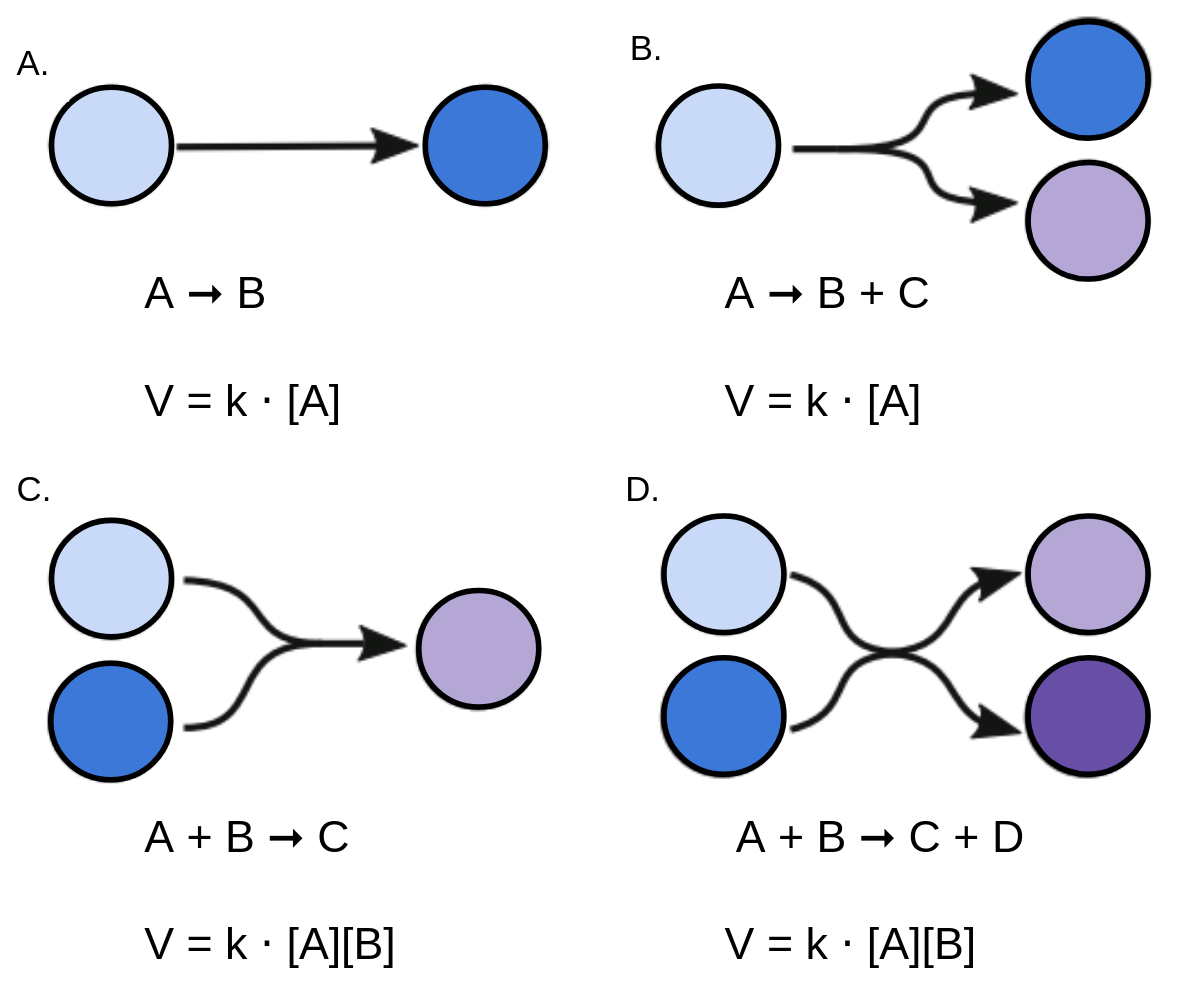
\includegraphics[width=7cm]{images/Reactions.png}
    \captionof{figure}{Models were composed of four reaction types and rate laws: (A) uni-uni, (B) uni-bi, (C) bi-uni, (D) bi-bi}
    \label{fig:reaction}
    
\end{figure}





\subsection{Model Representation}

Models and reactions were represented by custom data structures. An instance of the \textit{reaction} object represents a single reaction and consists of one or two reactants, one or two products, a rate constant, and an integer representing the reaction type (uni-uni, uni-bi, bi-uni, or bi-bi). The \textit{model} object represents a single reaction network and consists of a list of species, a list of initial concentrations, and a list of \textit{reaction} objects. The software converts \textit{model} objects into systems of ordinary differential equations which are then numerically solved to produce time series data of species concentrations. After the evolution process is complete, the models are converted to antimony~\cite{Smith2009}, a human readable model definition language.

\subsection{Objective Function}

The objective function minimized error between the candidate model's time course data and a series of points corresponding to the peaks and troughs of an oscillator. This "idealized" oscillator time series consisted of nine concentration points, alternative between 5 and 30 concentration units over the course of 1.25 seconds (figure \ref{fig:fitness}). The output time series of each species was compared to these points by summing the squared difference between the observed point and the "ideal" point and the smallest error value was considered the model's fitness. This is similar to MSE but the sum is not divided by the number of observations as this number is constant across all models. This has been demonstrated to be an effective objective function for the in silico evolution of chemical oscillators~\cite{Paladugu2006}.  In cases where candidate models could not be simulated, an arbitrarily high fitness value was assigned resulting in their subsequent removal from the population in the selection step.  

\begin{figure}
    \centering
    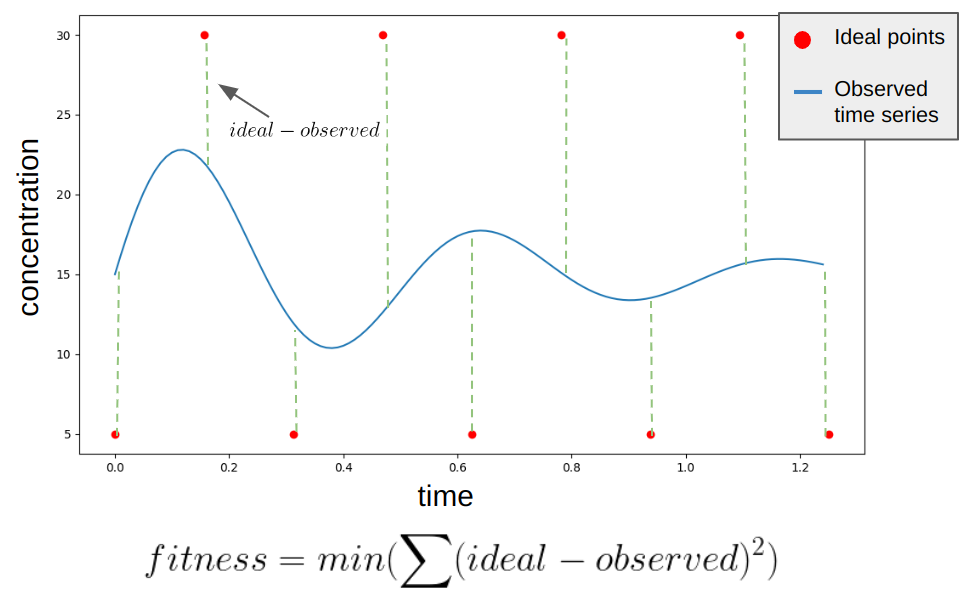
\includegraphics[width=10cm]{images/fitness.png}
    \captionof{figure}{For the time series data of this species, the error is calculated by summing the square difference between the observed time series data (blue) and a set of idealized oscillator points (red). This process is repeated for each species in the model and the fitness is defined as the minimum of these sums. }
    \label{fig:fitness}
\end{figure}

\subsection{ODE Solver}
Preliminary studies suggested that the most commonly used python ODE solver from scikit was inaccurate for solving these problems. Other off-the-shelf solvers lacked the ability to deal with the custom data structure encoding the models. The Sauro Lab's simulation software, RoadRunner~\cite{Somogyi2015}, was also unsuitable for this purpose due to the computational cost of frequently modifying and recompiling models for simulation. Many algorithms, such as RK4 are not robust enough for this work. For this reason, a custom simulator using the CVODE solver from the Sundials suite was used~\cite{hindmarsh2005sundials}. 

\subsection{Selection}
In each new generation, the top 10\% of models from the previous generation were copied without modification. The remainder of the new population was chosen by tournament selection~\cite{Miller1995} from the previous generation. This is where two models are randomly chosen from the previous generation (including from the top 10\% of models already carried over) and the model with the better fitness is mutated by adding or deleting a reaction, or by modifying a rate constant. The modified model is then appended to the new generation. 

\subsection{Mutation}
After tournament selection, the fitter model was either mutated by modifying a rate constant or adding/deleting a reaction with equal probability. In the case of rate constant modification, a random rate constant was adjusted by a random percentage between -15\% and +15\% of the rate constant's current value. This mechanism ensured that rate constants could not become negative, and there was no upper limit to their value. 

In the case of reaction modification, a reaction was either added or deleted with 50\%-50\% probability. If deleted was selected, a random reaction was removed from the model. If addition, a new reaction was added with the equal probability of each reaction type: uni-uni, uni-bi, bi-uni, bi-bi (figure~\ref{fig:reaction}). 

\subsection{Random Networks for Evolution}
A population of 40 random networks were generated using the {\tt teUtils} python package~\cite{SauroteUtils_2020}. Each network was initialized with three species, and nine reactions with the probability of each reaction type being 0.1, 0.4, 0.4, 0.1 for uni-uni, uni-bi, bi-uni, and bi-bi reactions. These settings were chosen to maximize the number of evolution trials that successfully product oscillators. All reactions had mass-action kinetics with a random rate constant between 0 and 50. 
\begin{figure}
    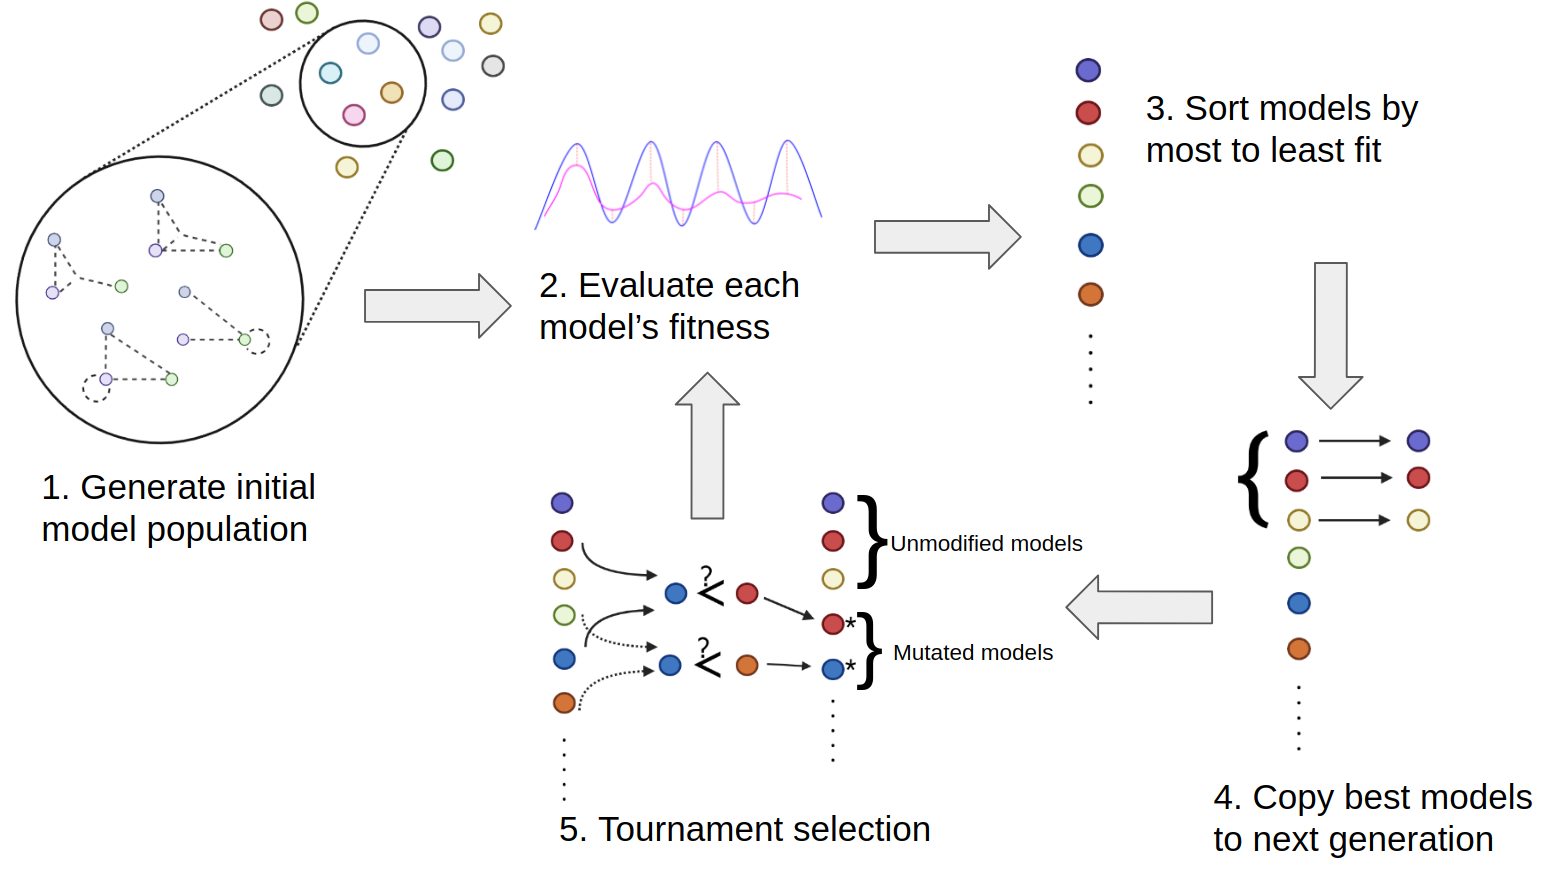
\includegraphics[width=12cm]{images/algorithm.png}
    \captionof{figure}{The evolution algorithm. (1) An initial population of random models is created. (2) The fitness of each model is evaluated. (3) The entire population is sorted by most fit to least fit. (4) The top 10\% of the models are transferred to the subsequent generation unmodified. (5)  Tournament selection is used to populate the remainder of the subsequent generation. Models are randomly selected, the more fit model is chosen to be modified and carried over to the subsequent generation. Steps 2-5 are repeated. }
    \label{fig:algorithm}
\end{figure}

\subsection{Custom Evolution Algorithm}

The evolutionary algorithm mimics biological evolution in that populations of individuals, in this case candidate networks, are altered and forced to compete with each other. Over the course of generations, fitter individuals (models that oscillate or are likely to oscillate) out compete unfit individuals (models that do not oscillate or can not be simulated) and survive into the next generation. Although genetic and evolutionary algorithms are well characterized, their application to systems biology models remains a challenge as a key trait in these algorithms is crossover, the ability of two possible solutions to exchange information, creating a new, ideally more suitable, candidate solution~\cite{Katoch2020}. Typically, genetic algorithms operate on objective functions for which solutions consist of vectors where values can easily be exchanged between two vectors. It is uncertain how crossover of mass-action kinetic models could be achieved as solutions (candidate networks) consist both of topology (how reactions are connected) as well as rate constants (vectors of values). Additionally, the number of reactions and rate constants vary and must be equal but can vary from model to model. For this reason, a custom optimization process was developed based on genetic algorithms but avoiding crossover. 

This process begins with the generation of 40 random networks with pre-specified probabilities for each of the four reaction types.  The fitness of each model is evaluated by comparing the model's time series data with an objective function representing the desired outcome, oscillation. Models that with time series data close to this desired outcome, those that oscillate or those with damped oscillations, are more fit than those that fail to oscillate or cannot be simulated. 

These models are ordered from most to least fit and the top 10\% of the models are carried over unmodified to the subsequent generation (figure \ref{fig:algorithm}). The remaining models are randomly paired and compared and the fitter of the two models is slightly modified by either adding or deleting a reaction or changing a rate constant. If the modification improves the fitness of the model, the modified model is added to the next generation. If the modification makes the model less fit, 75\% of the time the unmodified model is added to the next generation and 25\% of the time the less fit model will be added. This allows for the chance that small changes initially make a model worse, but subsequent changes drastically improve the model. Once the new generation is fully populated, the models are again ordered from most to least fit and the process begins again. This is repeated for 400 generations or until a threshold fitness level is reached.

\subsection{Random Control Networks}
Random models were generated as described in the previous section. To control for changes made during evolution, the random models underwent the same mutation processes described previously. Instead of populating subsequent generations based on model fitness, 10\% of the previous population was randomly selected to be carried over unmodified to the new generation. The remainder of the new generation was populated with models randomly chosen and mutated from the previous generation. The purpose of this procedure was to account for model variability introduced in the evolutionary process. Of 1000 random control networks generated, 1 was a spontaneous oscillator.

\section{Results}
Evolved models are processed to remove any undesirable oscillators from the population, namely oscillators that dampen over time or oscillators where one or more species concentrations rise indefinitely towards infinity. Next,  duplicated reactions were fused and reactions that are superfluous to oscillation are deleted to minimize network size resulting in a population of reaction networks that oscillate indefinitely in species concentration, examples of which are shown in figure 4.

\begin{center}
    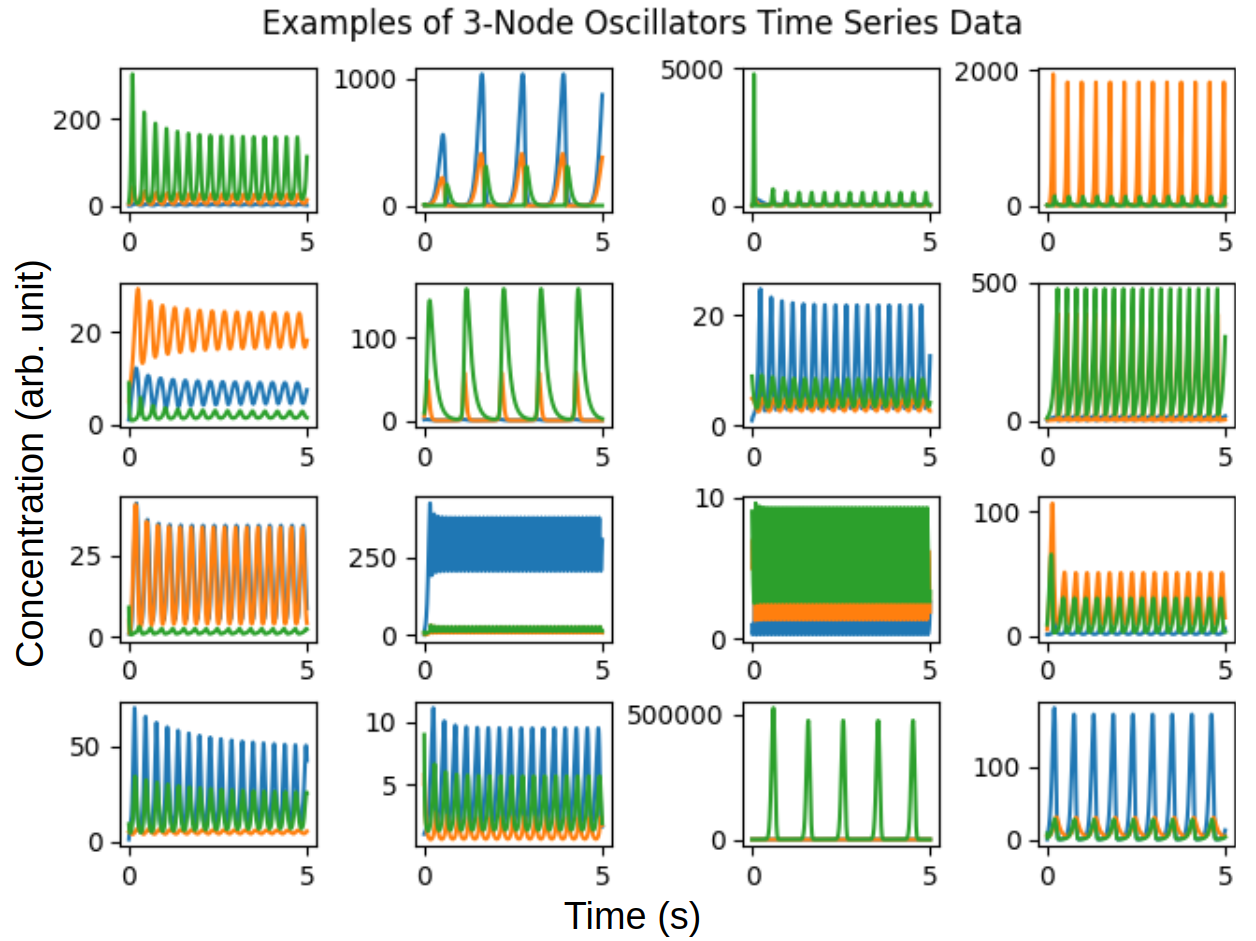
\includegraphics[width=8.5cm]{images/examples.png}
    \label{fig:examples}
    \captionof{figure}{Time series data of sixteen 3-node oscillators generated using differential evolution.}
\end{center}


\subsection{Database Construction}
A non-relational key-value database was deployed via Mongo Atlas using the PyMongo API to store all models and their information. The user enters the desired reaction network attributes into the web GUI (figure \ref{fig:website}). Models are downloaded as a .zip file of text files, or if a single model a single text file, containing the antimony string of each model. If the "Download in simulatable Tellurium form" box is checked, then each model file will contain the necessary python package imports and formatting to be immediately simulated and plotted upon running the file.


The current website queries the database by model type (current options are oscillator or random), the number of nodes (species), the number of reactions, and the presence or absence of autocatalysis or degradation reactions. Both oscillator and non-oscillating control networks are stored in the database. Each entry also includes a dictionary of tallies of each reaction type in the network, a list of redundant reactions that were fused during post-processing, a list of reactions that were deleted as their presence did not influence oscillation. 




In addition to the Antimony string comprising the model, other characteristics such as its initial reaction probabilities, fused and deleted reactions, and reaction counts are also tracked in the database.  The database can be queried to select models with any number of desired traits. Both oscillator and non-oscillating control networks are stored in the database.

The Cesium database is publicly available on the web at \url{https://cesiumdb.herokuapp.com/} and is intended to serve as source of reaction networks with specified characteristics for use in research and validation.  It currently contains 2000 randomly generated models and approximately 1800 3-species oscillating networks. This database can be expanded in the future to include a wider variety of oscillatory networks as well as networks with different behaviors, such as bistability. 

\begin{figure}
    \centering
    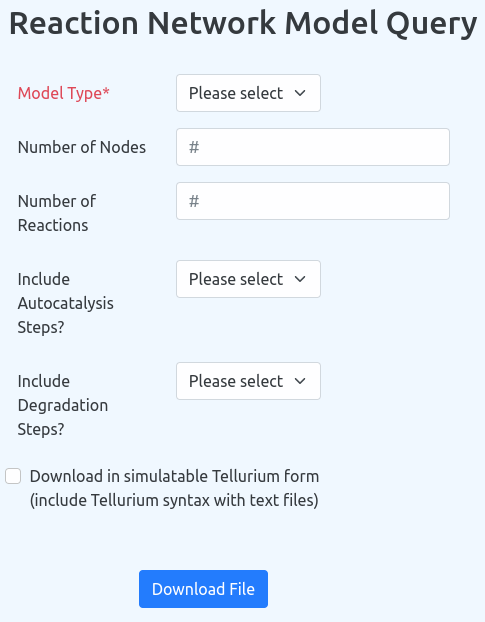
\includegraphics[width=8cm]{images/website.png}
    \captionof{figure}{Landing page for the Cesium database.}
    \label{fig:website}
\end{figure}

\subsection{Oscillating Network Examples}
Four oscillating networks from the database are shown in figure \ref{fig:model-diagrams}. Arrows symbolize reaction and lead from the reactant to the product. A double headed arrow indicates two products are formed and a double tail indicates two reactants. 


\begin{figure}
    \centering
    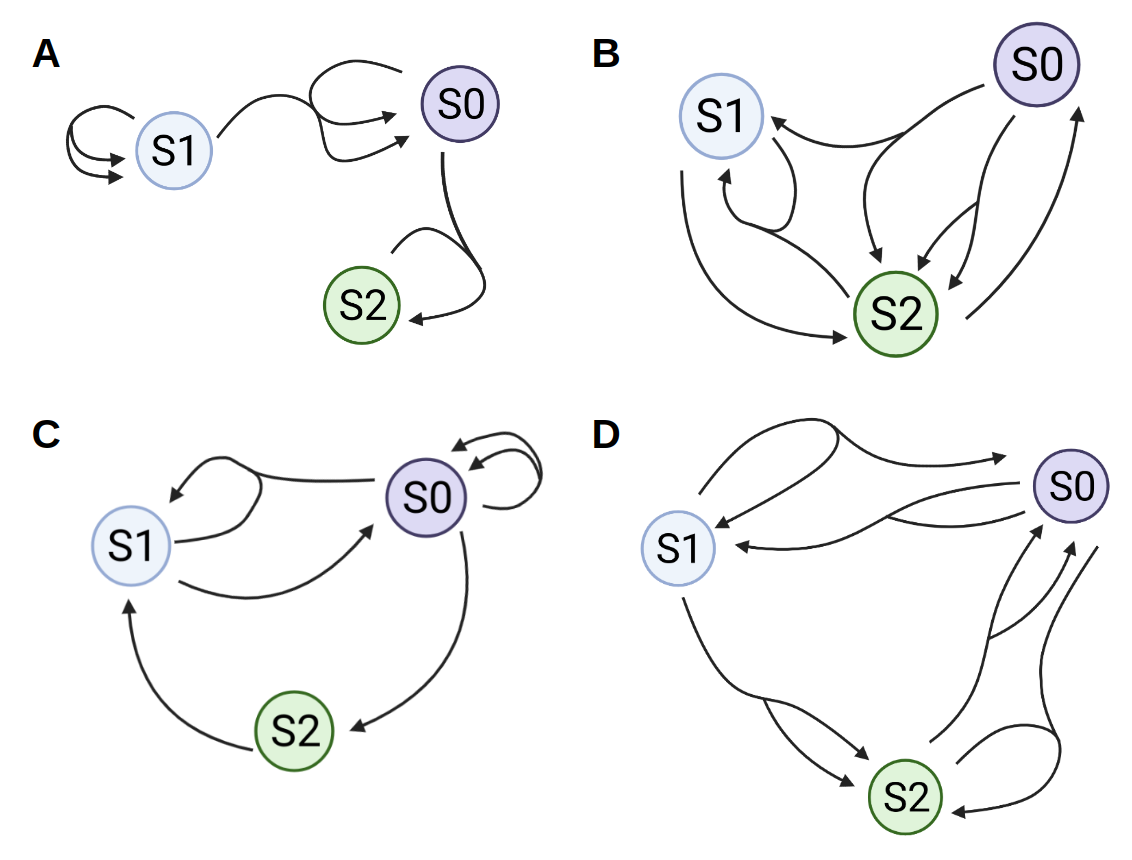
\includegraphics[width=8cm]{images/model-diagrams.png}
    \captionof{figure}{Examples of 3-species oscillating networks from the Cesium database.}
    \label{fig:model-diagrams}
\end{figure}

In network A, S1 is autocatalytic as is S0 (and catalyzed by S1). These linked positive feedback loops cause oscillation with products out flowing to S2, which essentially behaves as a boundary species, a species that is unaffected by the model and whose concentration remains fixed.  Network B lacks autocatalytic reactions completely. Computing the jacobian matrix at the unstable focus results in the following matrix:
\[
\begin{blockarray}{cccc}
S0 & S1 & S2 \\
\begin{block}{(ccc)c}
  -4.75 & 0 & 15.2 & S0 \\
  0.75 & -0.3 & 0 & S1 \\
  8.75 & -1.6 & -22.8 & S2 \\
\end{block}
\end{blockarray}
 \]
In the bottom row center, the negative number indicates that there is an inhibitory relationship between S1 and S2. An increase in S2 will decrease the production rate of S1. These interactions for a cycle with negative feedback, suggesting that this is a feedback oscillator (figure \ref{fig:feedback}). Similar analyses reveal that networks C and D are also likely to be feedback oscillators.

\begin{center}
    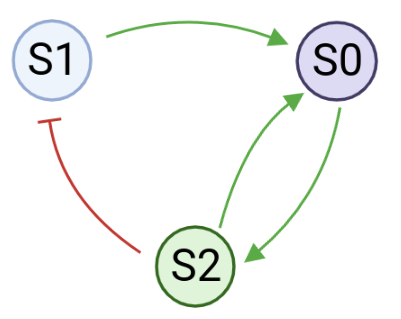
\includegraphics[width=5cm]{images/feedback-cycle.png}
    \captionof{figure}{Species interactions of Network B. Green arrows indicate activation and blunt red arrows indicate inhibition. The interactions form a cycle with negative feedback suggesting that Network B is a feedback oscillator.}
    \label{fig:feedback}
\end{center}


\section{Discussion}

Oscillating models were significantly enriched for autocatalytic reactions compared to control networks. Most oscillators are associated with unstable steady states. Destabilizing processes can be classified as 1) direct autocatalysis, 2) indirect autocatalysis (a positive feedback loop), and 3) end-product inhibition (a negative feedback loop)~\cite{Tyson1975, tyson2007}. Reactions are considered autocatalytic when the products increase the rate of reaction or when a chemical decelerates the rate of its own destruction~\cite{Tyson2004}. Given the two types of oscillators, negative feedback and negative feedback coupled with positive feedback~\cite{Sauro_dynamics}, it is unsurprising that autocatalytic reactions are enriched in the oscillator population as these reactions are a form of positive feedback. The portion of models containing at least one autocatalytic reaction in the oscillator and control populations were compared using a two-way chi square test. Of the 586 oscillating models, 83.1\% (487 of 586) contained an autocatalytic reaction compared with 49.8\% (498 of 1000) of the control models, a significant difference ($p < 0.0001$). 

Given the enrichment of autocatalytic reactions, one might expect a similar enrichment of degradation reactions, reactions where one species is removed from the system (eg. $X + Y \to Y$, where $X$ is removed from the system), to prevent species concentrations from rising to infinity. Interestingly, the presence of degradation reactions were not enriched in oscillating models. Of the oscillating model population 79.4\% (465 of 586) contained at least one degradation reaction compared to 76.3\% (763 of 1000) of the control models, an insignificant difference suggesting that although autocatalysis is a common characteristic in oscillating networks, degradation reactions are not necessary to prevent species concentrations from rising to infinity.  Although the presence of both an autocatalytic and a degradation reaction are not necessary for oscillation, it is rare that an oscillator contains neither. Only 0.5\% (3 of 586) of the oscillators analyzed had neither an autocatalytic reaction nor a degradation reaction compared to 0.2\% (2 of 1000) random models, an insignificant difference.

To determine if any reaction types were enriched in the oscillator population compared to the control population, the average model compositions were compared. The average model composition was assessed as the average number of reactions of the specific type were divided by the average total number of reactions for each group. For example, there were an average of 6.592 reactions per model in the oscillator population, of which an average of 0.99 were uni-uni reactions, for an average of 15.3\% uni-uni reactions in the average oscillator model (Table \ref{fig:avg-comp}). Compositions were compared with permutation tests, showing that model compositions and sizes were significantly different between the oscillator and control populations (the reduced size of oscillating networks can be accounted for by the fusion of duplicate reactions). Oscillators possessed significantly more uni-bi reactions compared to random control models. This is consistent with the enrichment of autocatalytic reactions which are often uni-bi. However, autocatalytic reactions can also be bi-bi reactions, which were not enriched in oscillating models. Although bi-bi reactions were less likely to be created during evolution due to the initial settings (10\%), it is somewhat surprising that bi-bi reactions were decreased in oscillatory networks given that a bi-bi reaction is slightly more likely to be autocatalytic ($\frac{4}{27}$) compared to a uni-bi reaction ($\frac{1}{9}$).

\begin{center}
    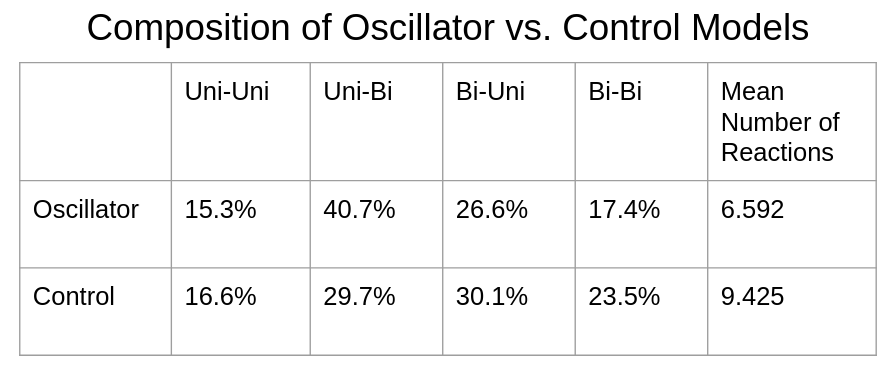
\includegraphics[width=8cm]{images/composition.png}
    \captionof{table}{Average reaction compositions of oscillating networks compared to non-oscillating controls.}
    \label{fig:avg-comp}
\end{center}

Next, oscillators containing autocatalytic reactions (498 models) were compared to oscillators lacking them (98 models). Populations were compared by permutation test. There was a significant increase in the portion of uni-bi reactions and a significant decrease in the portion of bi-uni reactions in non-autocatalytic models as compared to autocatalytic oscillators (Table \ref{fig:autocatal}). This result is interesting given that autocatalytic reactions are either uni-bi or bi-bi and both reaction types were reduced in oscillators with autocatalytic reactions compared to oscillators without. It is possible that oscillators without a single autocatalytic reaction are achieving autocatalysis through a combination of non-autocatalytic reactions.

\begin{center}
    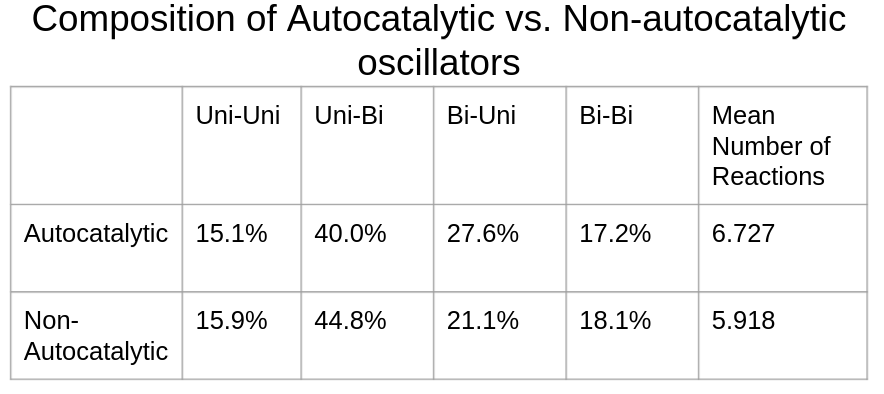
\includegraphics[width=8cm]{images/autocomp.png}
    \captionof{table}{Average reaction compositions of autocatalytic oscillating networks compared to non-autocatalytic oscillating networks.}
    \label{fig:autocatal}
\end{center}

Several manually inspected oscillators had reactions with extremely high rate constants (greater than 300, whereas most rate constants were between 5 and 75). The initial range for rate constants is 0 to 50 and with each mutation, they can only increase a maximum of 15\% of the current value. Although there is no upper limit for rate constants, it is nearly impossible to mutate a rate constant from the initial range to over 100 during the course of evolution. To bypass this limit and achieve high rate constants, many successful models have simply duplicated reactions during the evolutionary process. During post-processing, these duplicate reactions are fused and their rate constants summed. Fusing duplicate reactions to achieve high rate constants accounts for the observation that oscillators generally have fewer reactions than non-oscillators in this study. These high rate constant reactions can not be removed, nor can the rate constant be significantly lowered without impacting oscillation. Further investigation is needed to determine what essential function these high rate reactions seem to play in most of the oscillators included in this study. 


These oscillatory models and the random control networks have been added to a database, accessible at \url{https://cesiumdb.herokuapp.com/}. Models can easily be selected by the number of species, the number of reactions, and the present of autocatalysis or degradation reactions. The selected models can be downloaded in a zip file containing a .txt for each model. Each .txt file contains an individual model's antimony string. If the "Download in simulatable Tellurium form" option is selected, the .txt file will also contain formatting and package imports allowing the model to be easily simulated when the file is run as a python script. 

In the future, this database will be expanded to contain a variety of models with different behaviors besides oscillation. It is our hope that this database serves as a resource for the modeling community to study network behaviors and test novel software.


\section*{Funding}
This project was supported by National Institute of Health grant U01 CA238475 and the National Institute of Biomedical Imaging and Bioengineering for grant P41GM109824.

\section*{Acknowledgements}
We thank Lucian Smith for valuable discussions on differential evolution and model topology. 
\\
\\
This chapter was adapted from the following publication:
\\
\textbf{Tatka, L.}, Luk, W., Hellerstein, Elston, T., J., Sauro, H. “Cesium: A Public Database of Evolved Oscillatory Reaction Networks.”  Biosystems, vol. 224, 2023, p.104836., \\
https://doi.org/10.1016/j.biosystems.2023.104836. 
\\


\chapter{This is my next paper with a clever title}
Genetic algorithms (GAs), inspired by the principles of natural selection and genetics, have emerged as a powerful computational technique for solving optimization and search problems.Developed by John Holland in the 1960s, GAs mimic the process of biological evolution to solve optimization and search problems. At their core, genetic algorithms operate on a population of potential solutions, represented as individuals or "chromosomes," each encoding a candidate solution to the problem at hand. Through iterative generations, genetic algorithms apply mechanisms of selection, crossover, and mutation to evolve and refine the population, gradually converging towards optimal or near-optimal solutions. Selection favors individuals with higher fitness, mirroring the process of natural selection, while crossover and mutation introduce variation and diversity into the population, allowing for exploration of the solution space. By leveraging the principles of evolution, genetic algorithms offer a versatile and robust approach to solving complex problems across various domains, from engineering and optimization to biology and beyond.


Applying GAs to problems of parameter optimization is fairly straightforward as ``chromosomes" can be sequences of values, easily mutated and crossed over with other strings of values. This approach becomes more complex when applied to network problems, where network topology is deeply intertwined with parameter values. In these problems, the challenges becomes innovating while preserving decent candidate solutions. Stanley and Miikkulainen addressed this problem in 2002 with NEAT (NeuroEvolution of Augmenting Topologies), a powerful algorithm used for evolving artificial neural networks (ANNs). Unlike traditional methods of neural network training, which typically involve adjusting the weights and biases of fixed network architectures, NEAT evolves both the structure and weights of neural networks simultaneously.

At its core, NEAT employs a genetic algorithm to evolve populations of neural networks. Each individual in the population represents a neural network with its own unique topology (i.e., arrangement of nodes and connections). NEAT starts with a population of simple neural networks, often with minimal structure, and evolves them over generations to solve a given task.

One of the key innovations of NEAT is its ability to handle the complex task of evolving neural network topological structures. NEAT accomplishes this by employing three main mechanisms: speciation, historical marking, and structural innovation. Speciation encourages diversity within the population by comparing individuals against similar individuals as opposed to the entire population. This shelters innovations that may be weak at first, but will develop into robust solutions over several generations. A historical record of topological innovations serves as a "chromosome" and enables meaningful crossover without computationally expensive matching procedures required in other algorithms. Lastly, NEAT allows for the introduction of new structural innovations in neural networks through mutation. New nodes and connections can be added to existing networks, providing the potential for incremental growth and improvement over successive generations.


Systems biologist are no strangers to genetic algorithms. 

The similarity between ANNs and genetic regulatory networks was not lost on Dinh et al, who adapted this technique to getic

Francois and Hakim (Design of genetic networks with specified function...) were among the first to apply genetic algorithms to systems biology. They were trying to create small gene networks that functioned as either bistable switches or oscillators. Their algorithm only involved mutation and selection. For oscillators, they used the same objective function that I'm using here. Seems to have worked pretty well encourging further exploration in this space

Fujimoto et al looked at oscillaotry gene regulatory networks in the context of creating striped body pattens in developing drosophila. Well really arthorpods in general it seems. Similar approach to Francois and Hakim.

Kobayahsi et al also look at evolving oscillatory genetic networks. They fix parameter values and only allow connection rewiring to achieve oscillatory function. They wanted to look at statisticsal properties of genetic networsk as a relationship to oscillation period. THey only allow inhibitory reactions and thus all designs are essentailly extended versions of the three-gene repressilator circuit.

Deckard and Sauro expanded this concept beyond genetic regulatory networks to evolve small networks with specicfic computational capabilites such as square root and cube route calcultors. As with the previously mentioned algorithms, their alogrithm only uses mutation. They tried using crossover and it did not result in fitter offspring. They speculated that this was due to crossing over heterologous networks instead of homologous networks.

THis work was continued by Paladugu et al seeking to generate mass-action network functional modules with specific behaviors, including oscillators. The evolution algorithm used the addition or deletion of reactions or modification of rate constants as mutation operators. This algorithm avoided crossover as the authors argued that it would be disruptive.

Marchisio and Stelling argued that brute force optimization algorithms lack efficiency and that implementing some element of rational design could spped up automatic design of genetic networks implementing boolean logic gates. They separate structural and parameter optimziation by first generating several possible circuits and then ranks feasibility based on the structure. THen the best solutions undergo parameter optimziation. Separating structural design from parameters optimziation certainly saves computation time, but it relies on the existence of a rational solution, and is better suited for genetic networks, where these attributes are more easibly separated.



\section{Existing Software}

Although there are numerous studies implemting genetic algorithms in systems biology applications, few software packages exist to aid in this pursuit. In 2008, Kratz and Krishna developed GeNESis, a C based software with GUI to enable evolution of gene regulation networks. Its purpose was to help researchers undersatnd the evoltuionary behavior of populations of genetic regulatory networks. Connections were represented by binary strings, enabling the use of crossover. The URL to this tool is currently inactive.

Chandran and Sauro devloped a C library with basic functions for evolution of biological networks including genetic networks, protein networks, and mass-action networks. Although highly versatile, the library requires some C programming knowledge in order to customize the evolutionary algorithm.

\section{Evolving Reaction Networks}
The purpose of this work it twofold: (1) to create a general purpose, easily customizable, module for evolving mass-action chemical reaction networks and (2) to explore the effects of crossover,  speciation, and other hyperparameters on the success rate of the algorithm. Oscillatory chemical reaction networks were chosen as the target result of the evolutionary algorithm due to their biological relevance, poorly understood architectures (??), and the presence of intermediary states (damped oscillations) which aids in gradual evolution.
----

Oscillatory behavior is useful in a variety of biological processes including p53, circadian rhythm, and cell cycle. But also, you might want to generate oscillators as a component in a syntehtic biology ciruit. But really, this isn't about oscillators, that's just the test case. You might want a certain behavior and don't know how to build a  network to get it. Well This algorithm is for you! 

Other people have done similar things, but this is different. It starts with the concept of genetic algorithms, way back in 1975. These are algorithms to come up with optimization solutions. The algorithms kind of look like biologic evolution. You have a bunch of individuals, the fitter individuals share their genes and reproduce, less fit individuals die off, sometimes mutations occur and these can be either good or bad. Since then, the concept of genetic algorithms has been thoroughly explored, but here we present something slightly new. And that's how I'm going to get my PhD lol.

This all starts with the NEAt algorithm which is a way of evolving neural networks to do stuff.  What's interesting about this is they claim to have meaningful crossover and they use speciation to protect innovation. Dinh et al somehwat adapted this appraoch to genetic circuits, but those are a much easier problem because they just have activation and inhibition. Here, I adapt this algorthim to mass-action networks. That's way harder because there is way more complexity. In the first case, you just have an edge that connects two nodes and a weight. In the second, you add that the edge can either be activating or inhibiting, but here we add that the edge could connect multiple nodes (in the case of everything beyond a uni-uni reaction) and the reaction weight depends on what nodes it connects. More on that later.

I need to go over a bunch of times that this was done for a similar thing. Just as a quick review


---------------------------------
Some review stuff


Evolutionary design of oscillatory genetic networks (Kobayashi 2010)
Wanted to evolve genetic oscillatory networks. Get a large population of them and then mine them for statistics about oscillators and network motifs. They have fixed parameter values though and only change connections (?). Looks like they are also trying to evolve oscillators with specific frequencies. They have a cost function which looks at periodicity




\section{Methods}
\section{Encoding}
The main difference between ANNs and chemical reaction networks is that edges (reactions) can connect more than two nodes (chemical species) and that weights represent biochemical rate constants. Also activation is different but idk if that's relevant.
A chemical reaction network is composed of a set of reactions and initial concentrations.  A reaction consists of one or two reactants, one or two products, a rate constant, and a boolean indicating if the reaction is active or not.














\chapter{Background: \\\textit{Adapting Credibility Standards to Computational Systems Biology}}


\section{Introduction}

As computing power rapidly increases, computational models become more intricate and an increasingly important tool for scientific discovery. In systems biology, where the amount of available data has also expanded, computational modeling has become an important tool to study, explain, and predict behavior of biological systems. The scale of biological models ranges from subcellular components~\cite{Wang2021} to entire ecosystems~\cite{Hassell2021}. Modeling paradigms include mechanistic models, rule-based systems, Boolean networks, and agent-based models~\cite{Bartocci2016}. This review will focus on mechanistic models of subcellular processes.

The Food and Drug Administration (FDA) defines model credibility as ``the trust, established through the collection of evidence, in the predictive capability of a computational model for a context of use''~\cite{FDAguidelines}. Model credibility is important in systems biology as models are used to guide experiments or to optimize patient treatment. This is particularly important given the increasing scale and intricacy of models. Reproducibility, the ability to recreate a model and data \textit{de novo} and obtain the same result~\cite{shin_standards_nodate}, is directly connected to credibility, but even reproducibility remains a challenge. It was recently discovered that 49\% of published models undergoing the review and curation process for the BioModels~\cite{BioModels2020} database were not reproducible primarily due to missing materials necessary for simulation, the availability of the model and code in public databases, and lack of documentation~\cite{tiwari_reproducibility_2021}. With some extra effort, an additional 12\% of the published models could be reproduced.  A model that cannot be reproduced is not credible. 

Due to the increasing importance of computational models in scientific discovery, the National Aeronautics and Space Administration (NASA), the FDA, and other regulatory bodies have developed standards to assess the credibility of models~\cite{babula_nasa_2009,FDAguidelines,Shepard2015}. These standards are somewhat vague and generally qualitative to accommodate the broad scope of models in these fields. However, mechanistic models in systems biology are relatively narrow in scope and are supported by a variety of standards for model encoding, annotation, simulation, and dissemination potentially enabling the development of a credibility standard for mechanistic systems biology models.

In this chapter, we discuss current systems biology modeling standards that could aid in the development of credibility standards, examine existing credibility standards in other scientific fields, and propose that current standards in systems biology and other fields could support the development of a credibility standard for mechanistic systems biology models.

\section{Current Standards in Systems Biology}

Klipp et al. describe standards as agreed-upon formats used to enhance information exchange and mutual understanding~\cite{Klipp2007StandardsIC}. In the field of systems biology, standards are a means to share information about experiments, models, data formats, nomenclature, and graphical representations of biochemical systems. Standardized means of information exchange improve model reuse, expandability, and integration as well as allowing communication between tools. In a survey of 125 systems biologists, most thought of standards as essential to their field, primarily for the purpose of reproducing and checking simulation results, both essential aspects of credibility~\cite{Klipp2007StandardsIC}.

A multitude of standards exist in systems biology for processes from annotation to dissemination. Although there is currently no widely used standard for model credibility, the development of this standard is likely to depend on existing systems biology standards, just as standards for model simulation are dependent on standards for model encoding. This section will summarize current standards relevant to model credibility including standards for ontology, encoding, simulating, and disseminating models.  Although standards also exist for graphical representation of systems biology models (SBGN)~\cite{SBGN} and representation of simulation results (SBRML)~\cite{SBRML}, these will not be discussed here as they are less relevant to the future implementation of model credibility standards. 

\subsection{Model Representation}
Having a commonly understood language for describing a model is essential in exchange, reproducibility, credibility. Without a common language to describe models, they cannot be simulated across different platforms or freely shared. For this reason, systems biology model representation has become standardized using XML-based languages SBML~\cite{Klipp2007StandardsIC, machado_modeling_2011}, CellML~\cite{CellML}, and BioPAX~\cite{demir_biopax_2010}. NeuroML~\cite{Gleeson2010}, similar to SBML and CellML, is used to represent neuronal models, but is beyond the scope of this proposal.  

\subsubsection{SBML}

The most widely used model format is SBML (Systems Biology Markup Language)~\cite{SBML, Finney2003, Klipp2007StandardsIC, machado_modeling_2011}. SBML is a XML-based language for encoding mathematical models that reproduce biological processes, particularly biochemical reaction networks, gene regulation, metabolism, and signaling networks~\cite{SBML, Kohl2011}. SBML encodes critical biological process data such as species, compartments, reactions, and other properties (such as concentrations, volumes, stoichiometry, and rate laws) in a standardized format. Annotations can also be stored in the SBML format. With its support by over 200 third party tools and its ability to easily convert to other model formats, SBML is the de facto language for systems biology models~\cite{Kohl2011, machado_modeling_2011}.

SBML models are composed of entities, such as species, located in containers that can by acted upon by processes that create, destroy, or modify~\cite{Keating2020}. Other elements allow for the definition of parameters, initial conditions, variables, and mathematical relationships. The SBML language is structured as a series of upwardly compatible levels, with higher levels incorporating more powerful features. Versions describe the refinement of levels. Most recently, SBML level 3 introduced modular architecture consisting of a set of fixed features, SBML level 3 core, and a scheme for adding packages that augment the core functionality. This allows for extensive customization of the language while enabling reuse of key features. Currently, eight packages are part of the SBML 3 standard. These packages extend the capability of SBML such as enabling descriptions of uncertainties in terms of distributions~\cite{Smith2020}, allowing for the encoding, exchange, and annotation of constraint-based models~\cite{Olivier2018},  rendering visual diagrams~\cite{Gauges2015}, among many others~\cite{Keating2020}. 


\subsubsection{CellML}
Similar to SBML but broader in scope, CellML is also an XML-based language for reproducing mathematical models of any kind, including biochemical reaction networks~\cite{Beard2009}. CellML models do not encode biological information explicitly in the model, but instead consist of mathematical formulations of biological processes~\cite{Wimalaratne2009}. This feature of the CellML language increases flexibility enabling the description of a wide variety of biological processes. CellML models are composed of several interconnected components~\cite{Mesiti} with each component containing at least one variable that is associated with physical units.  This enables CellML processors to automatically check equations for dimensional consistency. 


Both CellML and SBML use almost identical mathematical expressions in MathML, an international standard for encoding mathematical expression using XML~\cite{Caprotti1999}. CellML explicitly encodes all mathematics, such as ODEs~\cite{Smith2013}. It is more versatile than SBML, capable of describing any type of mathematical model. SBML defines reaction rates, which can be used to build rate rules and ODEs~\cite{Hucka2015}. There is more third party support for SBML and it is a semantically richer language compared to CellML~\cite{machado_modeling_2011, Smith2013}.


\subsubsection{BioPAX}
BioPAX (Biological Pathway Exchange) is an ontology, a formal systems of describing knowledge that structures biological pathway data making it more easily processed by computer software~\cite{demir_biopax_2010}. It describes the biological semantics of metabolic, signaling, molecular, gene-regulatory, and genetic interaction networks~\cite{demir_biopax_2010}. Whereas SBML and CellML focus on quantitative modelling and dynamic simulation, BioPAX concentrates primarily on quantitative processes and visualization~\cite{demir_biopax_2010, buchel_qualitative_2012}.  

BioPAX contains one superclass, Entity. Within the Entity superclass, there are two main classes: PhysicalEntity and Interaction. PhysicalEntity describes molecules, including proteins, complexes, and DNA, while the Interaction class defines reactions and relationships between instances of the PhysicalEntity class. Interactions can be either Control or Conversion, both of which are divided into several more detailed subclasses~\cite{demir_biopax_2010, buchel_qualitative_2012}. Like SBML, BioPAX is released level-wise with level 1 describing interactions, level 2 supporting signaling pathways and molecular interactions, and level 3 enabling the description of gene-regulatory networks and genetic interactions.

\subsection{Annotation}

As models grow more numerous and complex, there is an increasing need for a standardized encoding format to search, compare, and integrate them. While standards such as SBML and CellML provide information on the mathematical structure of a model, there is no information as to what variables and mathematical expressions represent. Simple textual descriptions of these representations are subject to errors and ambiguity and require text-mining for computational interpretation~\cite{Curtout2011}. Standardized metadata annotations address these issues by capturing the biological meaning of a model's components and describing its simulation, provenance, and layout information for visualization. The use of annotations improves model interoperability, reusability, comparability and comprehension~\cite{Gennari2021}. Annotations are enabled by systems biology specific ontologies~\cite{Wimalaratne2009} which define a common vocabulary and set of rules to unambiguously represent information~\cite{Noy2001OntologyD1}.
 
To avoid accounting for a variety of annotation formats and approaches, standard annotation protocols are necessary~\cite{Gennari2021}. However, despite the numerous standards and tools, annotation remains a challenge. For example, the ChEBI database~\cite{Hastings2015} has approximately 1,000 annotations for glucose. While more than one entry for each annotation can serve a purpose (some users may prefer to be more abstract in their annotations), this adds to the challenge of defining the purpose of a model and, therefore its credibility.  Additionally, annotations can be obsolete, inappropriate or incorrect, or provide insufficient information. Evaluating the quality of annotations would be essential in any credibility assessment for systems biology models. Some tools already exist for this purpose, such as SBMate~\cite{Shin2021}, a python package that automatically assesses coverage, consistency, and specificity of semantic annotations in systems biology models.

\subsubsection{MIRIAM}
 MIRIAM (Minimum Information Requested in the Annotation of Biochemical Models)~\cite{novere_minimum_2005} was developed to encourage the standardized annotation of computational models by providing guidelines for annotation. The MIRIAM guidelines suggest that model metadata clearly references the relation documentation (e.g. a journal article), that the documentation and encoded model have a high degree of correspondence, and that the model be encoded in a machine-readable format (such as SBML or CellML). Annotations should also include the name of the model, the citation for its corresponding journal article, the contact information of the creators and date of creation, as well as a statement about the terms of distribution. Additionally, models should have accurate annotations that unambiguously links model components to corresponding structures in existing open access bioinformatics resources. The referenced information should be described using a triplet, {data collection, collection-specific identifier, optional qualifier} and expressed as a Uniform Resource Identifier (URI), a unique sequence of characters that identifies a resource used by web technologies~\cite{berners2005uniform}. The optional qualifier field is used to describe relationships between the model constituents and the piece of knowledge with language such as ``has a'', ``is a version of'', ``is homologous to'', etc. 
 
\subsubsection{Systems Biology Ontology (SBO)}
SBO (Systems Biology Ontology) describes entities used in computational modeling~\cite{SBO, Curtout2011}. It defines a set of interrelated concepts used to specify the types of components specified in a model and their relationships to one another. Annotation with SBO terms allows for unambiguous and explicit understanding of the meaning of model components and enables mapping between elements of different models encoded in different formats~\cite{Curtout2011}. Both SBML and CellML support annotation with SBO terms.  SBML elements contain an optional sboTerm attribute~\cite{Curtout2011, Hucka2015, Wimalaratne2009}. 


\subsubsection{OMEX}
In order to harmonize the metadata annotations across models encoded in various formats, Gennari \textit{et al.}, with the consensus of the COMBINE (Computational Modeling in Biology Network) community, developed a specification for encoding annotations in Open Modeling Exchange (OMEX)-formatted archives. The specification describes standards for model component annotations as well as for annotation at the model-level, and archive-level~\cite{Gennari2021}. The specification describes annotation best practices and addresses annotation issues such as composite annotations, annotating tabular data and physical units, as well as provides a list of ontologies relevant to systems biology. Implementation of these specifications is aided by LibOMexMeta, a software library supporting reading, writing, and editing of model annotations. It uses Resource Description Framework~\cite{Decker2000} (RDF), an XML-based standard format for data exchange on the web, for representing annotations. It also makes use of several standard knowledge resources describing biology and biological processes such as ChEBI~\cite{Hastings2015}, a dictionary of small chemical compounds, and UniProt~\cite{Apweiler2004}, a database of protein sequence and functional information.

\subsubsection{Annotation in CellML and SBML}
 Both CellML and SBML have their own annotation protocols based on RDF~\cite{Wimalaratne2009}. The CellML language uses its own ontology for model annotation, a necessity due to the flexibility of the language~\cite{Beard2009}. The CellML Metadata Specification was developed parallel to the CellML language~\cite{Wimalaratne2009}. CellMLBiophysical/OWL ontology is composed of two categories: physical and biological~\cite{Wimalaratne2009}. The physical ontology describes physical quantitative information and concepts captured in the model's mathematical expressions. It is subdivided into processes, such as enzyme kinetics, ionic current, and rate constants, and physical entities, such as area, concentration, volume, and stoichiometry. The biological ontology provides description for processes, entities, the role of an entity in relation to a process, and the specific location of the entity in a biological system. Bioprocesses are divided into three subclasses: biochemical reactions, transport, and complex assembly. Biological entities include proteins, small molecules, and complexes. The biological roles subclass is composed of modifiers, reactants, and products. 

%Hacky BS spacer before BioModels.net to prevent text from flowing into margins
SBML also facilitates MIRIAM compliant annotation using RDF)~\cite{Swainston2009,Decker2000}. Annotations use \\BioModels.net~\cite{LeNovere2006} qualifier elements embedded in XML form of RDF~\cite{Hucka2019}. Each annotation is a single RDF triple consisting of the model component to annotate (subject), the relationship between the model component and the annotation term (predicate), and a term which describes the meaning of the component (object). These terms come from defined ontologies, such as SBO~\cite{SBO}. RDF annotation is supported by the software libraries libSBML~\cite{libSBML} and JSBML~\cite{Rodriguez2015}.



\subsection{Simulation and Parameter Estimation}
Information about a model alone is insufficient to enable efficient reuse. A variety of advanced numerical algorithms and complex modeling workflows make the reproduction of simulations challenging. Many modelers reproduce simulations by reading the simulation description in the corresponding publication~\cite{waltemath_minimum_2011}. This is time consuming and error prone and the published description of a simulation is often incomplete or incorrect. For these reasons, it is essential to define and include information necessary to perform all simulations.

\subsubsection{MIASE}
Guidelines for the Minimum Information About a Simulation Experiment (MIASE) were introduced to specify what information should be provided in order to correctly reproduce and interpret a simulation~\cite{waltemath_minimum_2011}. MIASE is a set of rules that fall into three categories: information about the model used in the simulation experiment must be listed in a way that enables reproduction of the experiment; all information necessary to run any step of the experiment must be provided; all information needed to post-process data and compare results must be included.  Along with MIRIAM~\cite{novere_minimum_2005} guidelines, MIASE compliance guarantees that the simulation experiment is true to the intention of the original authors and is reproducible. 

\subsubsection{KiSAO}
KiSAO (Kinetic Simulation Algorithm Ontology) is an ontology used to describe and structure existing simulation algorithms~\cite{Zhukova2011, Curtout2011}. It consists of three main branches, each with several subbranches. The first branch is Kinetic simulation algorithm characteristics, such as the type of system behavior or type of solution. The second in the kinetic simulation algorithm such as Gillespie or accelerated stochastic simulation. The third branch is kinetic simulation algorithm parameters which describe error and granularity, among other characteristics. 

\subsubsection{SED-ML}
Simulation Experiment Description Markup Language (SED-ML) is software independent, XML-based format for encoding descriptions of simulation experiments and results~\cite{bergmann_simulation_2018, Smith2021simulation}. To help modelers comply with MIASE rules, SED-ML describes the details of simulation procedures, including what datasets and models to use, which modifications to apply to models, which simulations to run on each model, how to post-process data, report, and present results can all be encoded~\cite{waltemath_minimum_2011}. Each algorithm mentioned in a SED-ML file must be identified by a KiSAO term~\cite{Curtout2011}. PhraSED-ML was developed to enable modelers to encode human readable SED-ML elements without the use of specialized software~\cite{choi_phrased-ml_2016}.

\subsubsection{PEtab}
Parameter estimation is common in modeling and simulation, which often requires running multiple simulations to scan the suitability of several parameter sets.  Although many parameter estimation toolboxes exist, they each use their own input formats. The lack of a standardized format makes it difficult to switch between tools, hindering reproducibility~\cite{Schmiester2021}.  PEtab is a parameter estimation problem definition format consisting of several files containing information necessary for parameter estimation, including the model (in SBML format), experimental conditions, observables, measurements, parameters, and optional visualization files~\cite{Schmiester2021}. A final PEtab problem file links all other files to form a single, reusable, parameter estimation problem. Following the success of PEtab, parameter estimation functionality was added to SED-ML~\cite{Smith2021simulation}.

\subsection{Dissemination}
Model reproducibility best practices describe dissemination as an essential part of reproducibility~\cite{porubsky_best_2020}. Sharing all model artifacts and documentation on open-source repositories allows independent researchers to reproduce, reuse, and understand the model. Several guidelines and archive formats have been developed to ensure that all relevant information necessary to reproduce a modeling result is easily accessible to the public.


\subsubsection{MIRIAM Curation Guidelines}
In addition to annotation guidelines, MIRIAM also provides guidelines for model curation, the process of collecting and verifying models. The aim of MIRIAM guidelines is the ensure that model is properly associated with a reference description (e.g. a journal article) and that it is consistent with that reference description, meaning that it reflects the biological process listed in the reference description. The model must be encoded in a public, machine-readable format such as SBML or CellML and comply with the associated encoding standard. The encoded model must be simulatable, including quantitative values for initial conditions, parameters, and kinetic expressions, and must reproduce relevant results when simulated~\cite{novere_minimum_2005}.

\subsubsection{FAIR}
More recently, the FAIR guidelines were published to improve the ability of computers to \textbf{F}ind, \textbf{A}ccess \textbf{I}nteroperate, and \textbf{R}euse models~\cite{Wilkinson2016} with minimal human interaction. FAIR defines characteristics that data resources should possess to assist with discovery and reuse by third-parties. Unlike most data management and archival guidelines, FAIR is a set of high-level, domain-independent guidelines that can be applied to a variety of digital assets. Each element of the FAIR principle is independent. 

For a model to be ``findable," it should be easy to find for both humans and computers. This requires describing and annotating data and metadata with unique identifiers that are registered or indexed in a searchable resource. Once the user finds the relevant model, it should be accessible: data and metadata should be retrievable by their identifiers using standard communications protocol. Metadata should remain accessible even when data are no longer available. Interoperability refers to the integration with other data and the ability to operate with various applications and workflows. This is enabled by the use of broadly applicable languages for model representation and annotation. As the ultimate goal of FAIR is to enable the reuse of data, the guidelines dictate that data and metadata should be associated with detailed provenance, meet domain-specific community standards (such as COMBINE archive format described below), and released with clear and accessible data usage license.


\subsubsection{COMBINE Archives}
COMBINE (COmputational Modelling in BIology NEtwork) is a formal entity that coordinates standards in systems biology.  To assist in this coordination, a MIRIAM compliant system for sharing groups of documents regarding a model was developed called the COMBINE Archive~\cite{schreiber_specifications_2020}. The archive is encoded in OMEX (Open Modeling Exchange format) and the archive itself is a ``ZIP" file. A COMBINE archive could contain files in several different standard formats including SBML, SBOL, and SED-ML among others. Additionally, every COMBINE Archive contains at least one file titled \textit{manifest.xml} that contains a list of all the files comprising the archive and describing their locations. An archive also may contain a metadata file, ideally conforming to MIRIAM and MIASE guidelines. The inclusion of all necessary protocols and data needed to implement a model enables distribution of models via a single file encouraging reuse and improving reproducibility~\cite{bergmann_combine_2014}.



\section{Credibility Guidelines in Systems Biology}

Although no standard for model credibility in systems biology exists, there are general guidelines aimed at improving the trustworthiness of models developed by the Committee on Credible Practice of Modeling and Simulation in Healthcare, a group formed by the U.S. National Institutes of Health~\cite{erdemir_credible_2020}. The purpose of these guidelines is to encourage the credible use of modeling and simulation in healthcare and translational research. These guidelines are qualitative and share many components with best practices for reproducibility. The term ``credible" was defined as  ``dependable, with a desired certainty level to guide research or support decision-making within a prescribed application domain and intended use; establishing reproducibility and accountability." These guidelines are qualitative and intended to cover a variety of modeling approaches and applications within the biomedical context (figure \ref{fig:10rules}). 

The credibility of a model should be evaluated within the model's context of use~\cite{erdemir_credible_2020}.
 To this end, the guidelines recommend using contextually appropriate data and evaluating the model (performing verification, validation, uncertainty quantification and sensitivity analysis) with respect to the context in which the model will be used. Any limitations should be listed explicitly. 

Borrowing from software engineering best practices, the guidelines also recommend the use of version control to track model and simulation development as well as extensive documentation of simulation code, model mark-up, scope and intended use. Models should also include guides for developers and users and conform to domain-specific standards~~\cite{erdemir_credible_2020}.

Different simulation strategies should tested to ensure that the results and conclusions are similar across various tools and methods. All modeling components such as software, models, and results should be reviewed by third party users and developers and disseminated widely.  


\begin{center}
    \captionsetup{type=figure}
    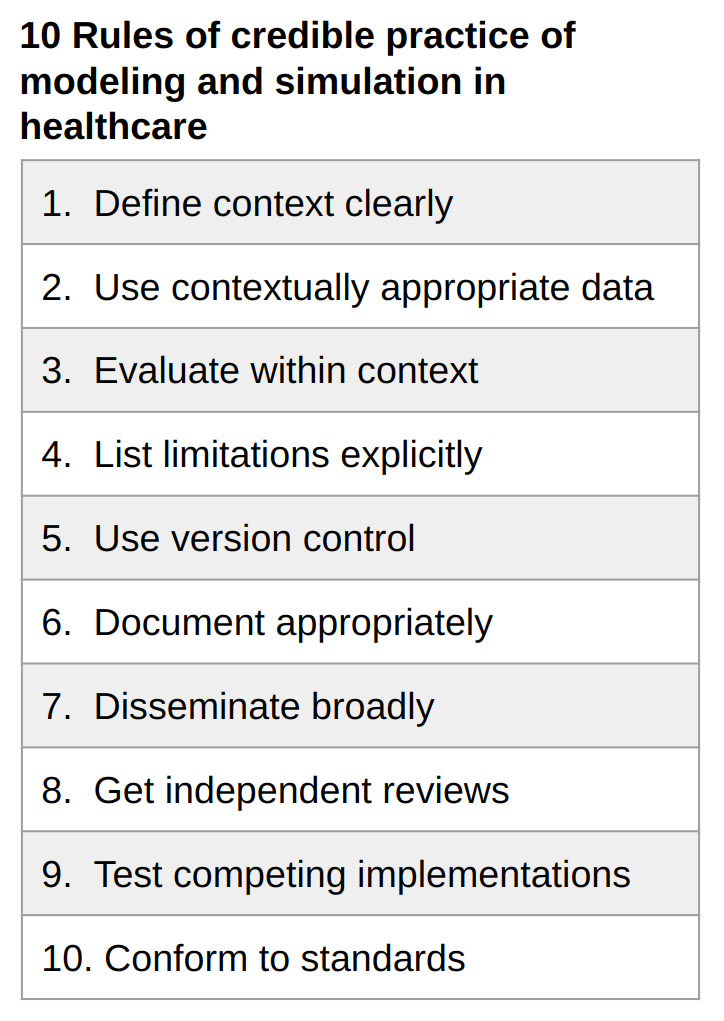
\includegraphics[width=6cm]{images/10rules.png}
    \captionof{figure}{The Committee on Credible Practice of Modeling and Simulation in Healthcare 10 rules of model credibility.}
    \label{fig:10rules}
\end{center}


\section{Qualitative Credibility Assessment in Other Modeling Fields}
NASA and the FDA also have a keen interest in producing well-documented and credible models for the purpose of making critical decisions. However, modeling and simulation tasks in these institutions are far broader compared to systems biology. NASA models range from the analysis of individual parts to orbits and spacecraft while models submitted to the FDA include medical devices and pharmacokinetics. Due to the wide variety of modeling tasks relevant to NASA and the FDA, credibility guidelines in these institutions are general, largely qualitative, and do not prescribe specific tests.


\subsection{NASA Credibility Assessment Scale}

After the loss of the Columbia Space Shuttle and its seven crew members in 2003, NASA significantly increased its focus on quantitative and credible models. The misuse of an existing model and the reliance on engineers' judgment led to the false conclusion that shuttle reentry would not be affected by a small hole in the heat shield caused by a debris strike during takeoff~\cite{Blattnig2013-qx, Howell2021}. The lack of quantifiable uncertainty and risk analysis in the report to management ultimately led to the shuttle's disintegration~\cite{Niewoehner2008}. Since then, NASA has developed extensive modeling and simulation standards including the Credibility Assessment Scale~\cite{babula_nasa_2009} (CAS) (figure \ref{fig:NASA}).  

Each model credibility standard described here emphasizes assessments be made within a specific context of use, the specific role and scope of the model and the specific question of interest that the model is intended to help answer~\cite{FDAguidelines}. The judgment error that ultimately led to the Columbia Space Shuttle disaster was partially due to the use of a modeling software far outside the intended context of use, leading to incorrect predictions and over-reliance on engineer's judgment~\cite{Blattnig2013-qx}. In addition to specifying the scope and question of interest, the context of us should also describe how model outputs will be used to answer the question of interest and whether other information, such as bench-testing, will be used in conjunction with the model to answer the question of interest~\cite{FDAguidelines}. The standards described here, from various institutions such as NASA and the FDA, all specify that credibility is to be evaluated within a specific context of use.

\begin{center}
    \captionsetup{type=figure}
    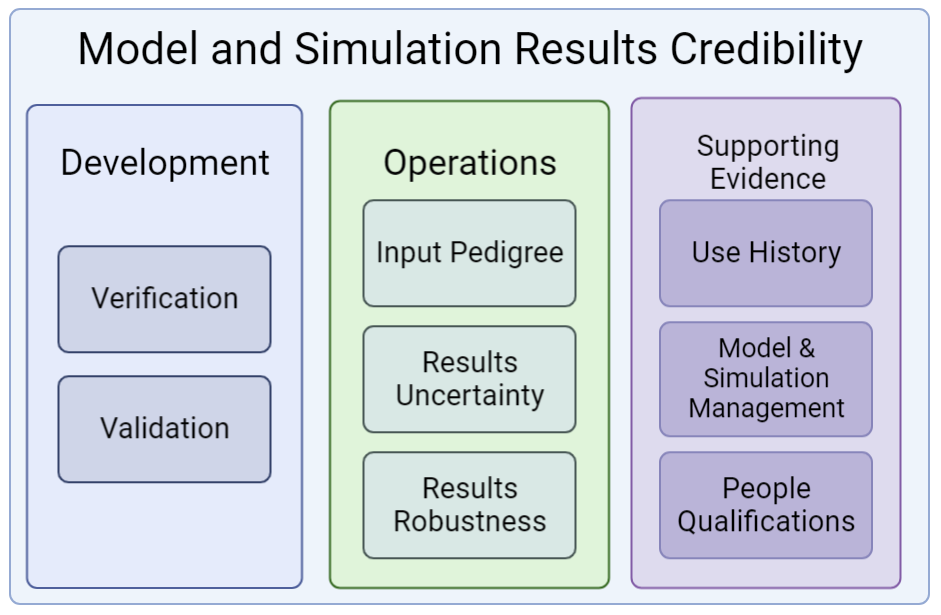
\includegraphics[width=8.5cm]{images/NASA_CAS.png}
    \captionof{figure}{Categories of the NASA Credibility Assessment Scale (CAS)}
    \label{fig:NASA}
\end{center}


NASA's CAS is intended to help a decision-maker evaluate the credibility of specific modeling and simulation results and to identify aspects of the results that most influence credibility~\cite{blattnig_towards_2008, Blattnig2013-qx}. The credibility assessment process can be viewed as a two part process: first the modeler conveys an assessment of the results, then a decision maker infers the credibility of these results. The CAS standard consists of eight factors grouped into three categories~\cite{babula_nasa_2009}: development, operations, and management. Each of the eight factors is scored on a scale of 0-4 with guidelines for each numeric score. These factors were selected as they were considered to be the most essential, sufficiently independent of one another, and could be objectively assessed. While the primary concern is the score for each individual factor, the secondary concern is the score of the overall model, which is the minimum score of the eight subfactors. 

The model and simulation (M\&S) development category consists of subsections verification and validation~\cite{babula_nasa_2009}. Scoring in these subcategories assess the correctness of the model implementation, the numerical error and uncertainty, and the extent to which the M\&S result matches reference data. If numerical errors for important features are ``small" and if results agree with real-world data, the highest score of 4 is awarded for these factors.

The second category, M\&S operations, consists of three factors: input pedigree, results uncertainty, and result robustness~\cite{babula_nasa_2009}. Input pedigree describes the level of trust in the input data, where input data that accurately reflects real-world data receiving the highest score. The results uncertainty category earns the highest score if non-deterministic numerical analysis is performed. Result robustness high scores are achieved by including sensitivity analysis for most parameters and identifying key sensitivities.

Model and simulation management, the third category, is less technical, containing the factors use history, M\&S management, and people qualification~\cite{babula_nasa_2009}. Use history scores the highest score if the model has previously been used successfully and meets de facto standards. For example, a model used for finite element analysis (FEA) would be required to meet FEA standards and codes for the type of object being modeled. M\&S management refers to the maintenance and improvement of the model with continual process improvement receiving the highest score of 4.  The people qualification category assesses the experience and qualifications of those constructing, maintaining, and using the model where personnel with extensive experience with the model and best practices scoring the highest. 

Although these categories were chosen, in part, due to their ability to be objectively assessed, there is still a significant subjective component of the scoring process. It is acknowledged that different decision makers may assign different degrees of credibility to the same model and different decisions may require different levels of credibility. The CAS serves as a template to assess and clearly communicate risks to decision-makers. Additionally, it can be useful in measuring model development progress or in identifying areas where improvement is most needed~\cite{Blattnig2013-qx}.


\subsection{Credibility Standards for Medical Models}
In addition to systems biology, computational models are also becoming essential tools in biomedical applications such as drug discovery~\cite{Chen2015}, pharmacokinetics~\cite{Kuh2000}, and medical devices~\cite{Kung2019}. Credibility is essential in biomedical modeling, particularly in cases where models influence patient treatment or regulatory approval of a device or drug. Both the FDA and the European Medicines Agency have developed standards guiding model credibility for the purposes of regulatory approval. As with NASA, these guidelines are broad and qualitative due to the broad scope of biomedical modeling. Before the FDA began formalizing guidelines for model credibility, the American Society of Mechanical Engineers (ASME) issued Verification and Validation (V\&V) 40 for assessing credibility of computational models in medical device applications~\cite{viceconti_credibility_2020}. However, this standard assumes the ability to perform traditional validation activities such as comparing model predictions to well-controlled validation experiments~\cite{FDAguidelines}, a task which can be unfeasible with some biomedical models. Many models used in regulatory submissions are supported by many sources of evidence beyond traditional validation experiments including clinical trials and population-level validation. Recognizing this fact, FDA modeling credibility guidelines expand on ASME V\&V 40 concepts to provide a more general framework for assessing a wider variety of models.


\subsubsection{ASME V\&V 40}

The ASME developed the V\&V 40 standard in 2012 as a means of describing verification and validation activities in the modeling and simulation of medical devices~\cite{viceconti_credibility_2020}. Like the NASA CAS, V\&V 40 focuses on context of use, model risk, and the establishment of credibility goals prior to any credibility assessment. The context of use addresses the specific role of the model in addressing the question of interest. Model risk is then assessed based on the possibility that the model may lead to incorrect conclusions resulting in adverse outcomes. After the establishment of credibility goals, verification and validation take place. 

Of particular relevance to modeling in systems biology are the descriptions of code and calculation verification found in V\&V 40. Verification seeks to determine if the model is built correctly. More specifically, code verification aims to identify any errors in the source code and numerical algorithms. This can be done by comparing output from a model to benchmark problems with known solutions~\cite{viceconti_credibility_2020}. Calculation verification estimates the error in the output of a model due to numerical methods. Output errors can include discretization errors, rounding errors, numerical solver errors, or user errors. Calculation verification is complete when it is demonstrated that errors in the numerical solution are minimized to the point that they are not corrupting the numerical results~\cite{viceconti_credibility_2020}.

Validation assesses how well the computational model represents reality. Validation activities might include comparing the model's behavior to the biological features of the real phenomenon by comparing results to \textit{in vitro/in vivo} benchmark experiments. Validation also includes uncertainty quantification and sensitivity analysis. Uncertainty quantification refers to the estimation of how stochastic error in the input propagates into the model's output. Sensitivity analysis is a post-hoc examination of the results of the uncertainty quantification to evaluate which elements most influence output variability~~\cite{viceconti_credibility_2020}.

Unlike the NASA CAS, V\&V 40 does not describe the quality of evidence needed to prove a model credible and lacks an objective scoring system necessary for implementing ``cut-offs" of credible versus non-credible models, or for comparing the credibility of multiple models.

\subsubsection{FDA Guidance on Computational Model Credibility in Medical Devices}

Based on the V\&V 40 standard, the FDA released guidance on assessing credibility for models of medical devices~\cite{FDAguidelines}. This guidance expands V\&V 40 to include other forms of credibility evidence beyond traditional verification and validation exercises. Applicable to physics-based, mechanistic, or other first-principles-based models of medical devices, these guidelines consist of ten categories broadly divided into code verification, calculation verification, and validation. The code verification category is taken directly from V\&V 40 described previously.

The calculation verification guideline extends the V\&V 40 by detailing several methods to verify that the model produces the intended output.  For example, the model results can be compared with the same data used to calibrate the model parameters. Broader evidence in support of the model, but perhaps without a specific context of use are also acceptable. A model can also be verified using \textit{in vitro} or \textit{in vivo} experiments either within the context of use, or within conditions supporting a different context of use. These techniques can also be used for validation evidence. 

Validation assesses the model's ability to reproduce real-world behavior. In addition to the methods described for calculation verification, validation can also include population-based evidence, statistical comparisons of model predictions to population-level data such as the results of a clinical trial. Credibility is also supported by emergent model behavior, the ability of a model to reproduce real-world phenomena that were not pre-specified or explicitly modeled, as well as general model plausibility, that model assumptions, input parameters, and other characteristics are deemed reasonable based on scientific knowledge of the system modeled. 

Unlike the NASA Credibility Assessment Scale, these FDA guidelines are sets of nonbinding recommendations. Additionally, no scoring or suggested quality measures of FDA credibility factors are included making quantitative analysis of credibility impossible.


\subsubsection{EMA Guidelines for PBPK Models}

Of particular relevance for the field of systems biology is The European Medicines Agency's (EMA) Guideline on the Reporting of Physiologically Based Pharmacokinetic (PBPK) Modeling and Simulation issued in 2018~\cite{viceconti2021, Shepard2015} . PBPK models are mathematical models that simulate the concentration of a drug over time in tissues and blood. With the rise in regulatory submissions that include PBPK models that rely on specialized software programs, this guideline provides detailed advice on what to include in a PBPK modeling report. 

The standard dictates the necessary information to describe and justify model parameters. Like the FDA standard, modelers are required to submit any assumptions made when assigning parameters and to document the sources of any literature-based parameters. Additionally, modelers must perform a sensitivity analysis for parameters that are key to the model (those that significantly influence the outcome) and list any parameters that are uncertain. 

The submission must include the simulation results as well as the files used to generate the final simulations in both tabular and executable format. This requirement is shared with reproducibility standards already in place for systems biology in the COMBINE Archive standard as well as described in systems biology modeling reproducibility best practices~\cite{porubsky_best_2020}.

The predictive performance of the model must also be evaluated. That is, its ability to recapitulate observed pharmacokinetics. This requirement is also mentioned in the FDA guidelines. 

Lastly, the guideline requires a discussion of uncertainty and confidence in the model. Although described more qualitatively in the EMA standard, this requirement is shared by NASA's CAS, V\&V 40, FDA credibility guidelines, and best practices for reproducible modeling in systems biology~\cite{porubsky_best_2020}.




\subsection{Current Tools for Systems Biology Model Testing}
Although there is no credibility standard in systems biology modeling, some tools provide automated model testing. Although these tools were not developed explicitly to assess credibility, many of the factors they test for could be considered aspects of credibility. Future model credibility assessments could aspire to the level of quantification and automation these tools offer. 
 
\subsubsection{MEMOTE}
MEMOTE (MEtabolic MOdel TEsts) is an open-source Python software that automatically tests and scores genome-scale metabolic models~\cite{Lieven2020-kj}. MEMOTE offers a web interface and command line interface where SBML files can be uploaded and analyzed, and ultimately scored. The tests check that a model is annotated according to the MIRIAM standard, that components are described using SBO terms, and that the model is properly constructed using the relevant SBML package, SBML-FBC~\cite{Lieven2020-kj, Olivier2018-tx}. Basic tests check for the presence of relevant components, charge information, and metabolite formulas. Biomass tests check that biomass precursors are produced and that the growth rate is non-zero. Stoichiometry tests test for inconsistency, erroneously produced energy metabolites, and reactions that are permanently blocked. A numeric score is output after testing indicating the extent to which a model conforms to these standards.

MEMOTE is designed to assess genome-scale metabolic models and largely includes tests that are specific to this model subset. Although a high MEMOTE score is likely to be indicative of model quality and reproducibility, it is not an assessment of credibility. A credible model will likely have a good MEMOTE score, but a good MEMOTE score does not necessarily indicate a credible model. However, the quantitative and automated nature of MEMOTE allows for quickly gauging model quality, comparing models, and the iterative improvement of metabolic models.

\subsubsection{FROG Analysis}
Similar to MEMOTE, the COMBINE community has recently developed FROG analysis, an ensemble of analyses for constraint-based models to generate standardized numerically reproducible reference datasets~\cite{sbmlsim21}. Results from constraint-based models are often communicated as flux values and there are often multiple solutions for a single model. As such, results cannot be used to gauge reproducibility. The COMBINE community outlined a list of outputs and results of flux balance analysis that are numerically reproducible and can be used for curation, known as FROG reports. FROG reports can be used in the BioModels~\cite{BioModels2018a, BioModels2020} curation process to assess reproducibility.

FROG analysis consists of  \textbf{F}lux variability analysis, \textbf{R}eaction deletion, \textbf{O}bjective function values, and \textbf{G}ene deletion fluxes. Flux variability analysis tests that the maximum and minimum fluxes are reproducible using different software tools. The objective function value for a defined set of bounds should be reproducible. The systematic deletion of all reactions or all genes, one at a time, should provide comparable reference results. Currently four tools support the generation of FROG reports. Web-based tools include fbc\_curation~\cite{sbmlsim21}, CBMPy MOdel Curator~\cite{SBMpy} (both of which are also available as command line tools), and FLUXER~\cite{hari2020}. fbc\_curation\_matlab is a command-line tool and exports results in COMBINE archive format~\cite{fbc_curation}.

Unlike MEMOTE, FROG analysis produces a report in lieu of a single numerical score. 

\section{Discussion}
When standards are established, tests can be established to assess the extent to which a model conforms to that standard. With the development of standardized quantitative metrics (as opposed to qualitative guidelines such as those discussed previously), models can be constructed to meet minimum quality requirements lending credibility to those models and allowing for easy comparison across models~\cite{Kaddi2007-js}. 

The difficulty in developing these quantitative metrics is that the characteristics of an ideal bio-model must be known and expressed concisely. Existing standards in systems biology seek to address the first point by outlining what information is necessary to completely define and reproduce a model as well as the format in which that information is to be presented. However, a model could meet all existing standards and not be credible. For example, a model could be fully defined in SBML with extensive annotations, be reproducible, properly formatted for dissemination with SED-ML files describing all simulations. Despite meeting these standards, this hypothetical model could produce negative concentrations when simulating, clearly indicating that the model is not credible.  Additional metrics and standards must be established to adequately assess credibility. These metrics might include the relative concentration of floating species or the shape of response curves.

Hellerstein \textit{et al.} note that several issues in biomedical modeling are analogous to problems faced in software development and propose that software development best practices might be translated to improve modeling in systems biology~\cite{Hellerstein2019}. Of particular interest is software testing, which can be considered a form of credibility assessment. These tests aim to ensure the correctness, reliability, and availability of software, all characteristics that are also essential in systems biology model credibility. 


Software tests can be divided into two categories, which may also be applicable in systems biology modeling: (i) black-box testing and (ii) white-box testing. Black-box software testing assesses the behavior of the code and does not deal with implementation. For systems biology model credibility assessment, black-box credibility indicators might be that the model accurately predicts observed data. White-box testing evaluates the internal workings of a software project or model. The absence of errors, such as undefined parameters, typos, or unused species, might serve as white-box credibility indicators.  



\section{Conclusion}

Although many reproducibility standards are in use to simplify assessing reproducibility, there are no standards and scoring systems for model credibility in systems biology. Unlike institutions such as NASA and the FDA, which deal with models spanning a broad scope of applications and scales, systems biology is focused on the modeling of cellular processes. This narrow scope, combined with the variety of standards already in use, makes systems biology models well-suited for a credibility standard.

A quantitative credibility scoring system would be particularly useful and enable comparing the credibility of different models and guide the development of more credible models. Credibility metrics could be published alongside models to indicate the trustworthiness of results and allow users to make informed decisions about reusing models.


Systems such as MEMOTE demonstrate that model standards and model quality indicators can be automatically quantitatively scored enabling iterative improvement during the development phase. More challenging is further developing standards to express characteristics, both quantitative and qualitative, that make a model credible. Current modeling standards in other scientific fields emphasize assessing credibility in the model's context of use. This poses a challenge for automating credibility assessment in systems biology modeling as more or less rigor may be required to achieve a sufficiently credible model depending on the intended use of the model. It may prove useful to develop a manual, semi-quantitative scoring systems, such as NASA's Credibility Assessment Scale prior to attempting to implement a fully quantitative and perhaps automated credibility scoring system for systems biology models.

\subsection*{Funding}
This work was supported by NIH Imaging and Bioengineering (NIBIB) award P41GM109824, and the National Science Foundation award 1933453. 
\\
\\
This chapter was adapted from the following publication:\\
\textbf{Tatka, L.}, Smith, L., Hellerstein, J., Sauro, H. “Adapting Modeling and Simulation Credibility Standards to Computational Systems Biology.”   Journal of Translational Medicine, submitted.

\chapter{Overview of Proposed Research:\\\textit{Software for Automated Credibility Assessment in Systems Biology Models}}

\section{Introduction}

As computational models grow in number and complexity, they become an increasingly important part of decision making processes. For this reason, it is essential that computational models be high quality, reproducible, and credible. Although other scientific fields are building qualitative guidelines for model credibility, no such standards exist for systems biology models. 

The purpose of this research is to create a user-friendly tool to automatically test systems biology models and assess their credibility. Users could access this software either online or locally via GUI or command line.  The user would input their model in a standardized format, such as SBML~\cite{SBML}, and the software would assess the model's structure and behavior, verify that the model's output is consistent across platforms, and validate the model against validation data provided by the user. The software would produce and overall score for model credibility as well as a report detailing areas where model credibility could be improved. This tool would be targeted at (1) modelers who may use this tool during the development process to iteratively improve their model (2) by journals or reviewers who may wish to verify a model is sufficiently credible for publication and (3) third parties who want to assess a previously published model's credibility prior to using it in their own studies or decisions.  


\section{Types of Software Testing}
The proposed credibility assessment tool will borrow from software testing best practices common in computer science. 
In particular, this software will make use of static, dynamic, and unit testing. The proposed research will focus on dynamic testing. Other members of the Sauro lab are currently developing static tests.

Static tests are tests that can be performed without running any code. In this context, static tests might include testing for errors in naming, ratelaws, or kinetics, nonsensical processes, uninitialized variables/parameters, relationships between species, and more. Model annotation may also be included in static testing. These test are beyond the scope of the proposed research, but will be included in the final software. 

Dynamic tests, the primary focus of this research proposal, assess a model's behavior and require that a model be simulated. These tests might examine the dynamics of model time courses, test for runtime exceptions, and ensure the species concentrations are within certain bounds.

Unit testing refers to the practice of testing small pieces of isolated code to ensure the correct output. Translating this concept to systems biology is less obvious as it is unclear what could be considered an isolatable unit. Perhaps a single reaction could be a unit. Tests might involve checking for errors in the rate law (i.e. that the rate law is dependent on at least one of the substrates), checking for mass balance errors, verifying correct annotate, and ensuring that there are no nonsensical reactions. 


\section{Sensitivity Analysis}
This proposal will also address parameter sensitivity as a metric for credibility. Parameter sensitivity refers to the extent to which a change in a parameter value influences change in the model output. A small change in a highly sensitive parameter value would lead to a large change in model output. Due to genetic variability, biological system parameters are slightly varied in nature. Nonetheless, biological systems remain functional across organisms despite these small variations. In general, a the presence of a highly sensitive parameter would indicate that a model is less credible.

\section{Research Aims}
This proposal is broken down into three primary aims discussed in detail in the following chapters. 

\textbf{Aim 1: Develop a python package to perform dynamic tests on systems biology models in order to assess their credibility.}\\
Initial dynamic tests will include testing that species concentrations do not become negative or increase to infinity, testing that specific changes in model variables affect the model output as intended, and checking if species concentrations are within pre-specified bounds.

\textbf{Aim 2: Create tools to automatically verify and validate models}. \\
Verification ensures that models perform consistently when simulated on different platforms. BioSimulations, a recently developed tool to encapsulate various simulators and operating systems, will be used to perform verification tests. Validation ensures that a model captures the experimental data it was intended to represent. Developing validation protocols is a greater challenge and will likely require that the user submit validation data alongside their model. 

\textbf{Aim 3: Build software to automate parameter sensitivity analysis.}\\
High parameter sensitivity increases uncertainty in a model's output and reduces model credibility.


\chapter{Dynamic Testing}
The field of software engineering has relied on static and dynamic testing for decades to ensure proper functionality~\cite{Fairley78}. In broad terms, static tests can assess code without executing the code whereas dynamic test require code execution\footnote{ It should be noted that the phrase ``dynamic testing" as used in this proposal refers to tests that require model simulation. It \textit{does not} refer specifically to tests of a model's dynamics, although confusingly, model dynamics are one subject tested with dynamic tests. }. Translated to computational systems biology, static tests assess a models structure and dynamic tests assess a model's behavior when simulated. Both are essential tools to ensure the functionality and credibility of a model, but \textbf{the scope of this proposal covers only dynamic testing.} Static tests are being addressed by other members of the Sauro Lab. In the long term, the proposed credibility test suite may be combined with static test suites currently in development.






\section{Model dynamics}
Unlike static tests, dynamic tests require simulating the model in order to check for things like enzyme behavior. Some essential dynamic checks are for species concentrations. Species concentrations shouldn't be less than zero as negative concentration is meaningless. Similarly, concentrations should not approach infinity over time as this is biologically impossible and clearly indicates either an error in the model or lack of model credibility. These checks might seem trivial, but they are simple ways of testing model credibility. One might think it is easy to simulate a model and see if there are negative concentrations or concentrations that approach infinity, but with an automated approach, a reviewer could easily assess the credibility of a model, a journal editor could run several models through the software to quickly check for these issues.

\section{Negative Concentrations and Concentrations Approaching Infinity}
In terms of implementation, checking for negative concentrations is relatively simple. The model would be simulated over a relevant timecourse, perhaps determined by units included in the model or drawn from figures, and then the timecourse data would be scanned to check for negative values. Very small negative values that are possibly results of machine precision errors would be flagged as a warning, while significant negative values would fail the test and alert the user. The presence of negative concentration values could indicate a simple typographical error in stoichiomety or rate constants, or could be indicative or a larger problem with the model. In either case, they signal reduced model credibility.

Concentrations that approach infinity are also indicative of poor model credibility. Like negative concentrations, concentrations approaching infinity could be due simple typos, or signal a larger problem with the model. Unlike negative concentration testing, tests for infinitely rising concentrations are less simple. As depicted in figure \ref{fig:infinity}, a model simulated for a short time period might show a species rising in concentration throughout the simulation, but when simulated for longer, the concentration may level out to a steady state or oscillate. Additionally, checking that a concentration never decreases during simulation is insufficient, as a concentration can oscillate while approaching infinity. Similarly, checking for ``unreasonably large" concentrations might yield false positives. For example, a concentration of $10^30$ g/mL would clearly be unreasonable, but if the concentration is given in molecules it becomes believable. Most likely a test to determine if concentrations approach infinity would need to be multifaceted.

The most straight forward testing technique would be to simulate the model for increasing amounts of time while testing for RuntimeErrors in the solver. When a model can be successfully simulated in smaller timescales, but causes the solver to fail at longer time periods, it is often indicative of a concentration that approaches infinity. Solver  errors typically arises when values are so large that the solver can't handle them. Unfortunately, ``small" timescales where the model simulates and ``large" timescales where it doesn't due to infinite concentrations are poorly defined and different across models. One model may rapidly approach infinity and fail when simulated for longer than 10 seconds while another might only fail after 500. 

Neither checking for simulation errors nor checking for species that fail to decrease or reach steady state are sufficient to test for concentrations that approach infinity. It may be possible to check for this mathematically, but implementation would be a challenge. While insufficient, perhaps the combination of multiple tests would be able to flag suspect concentrations for manual inspection.


\begin{center}
    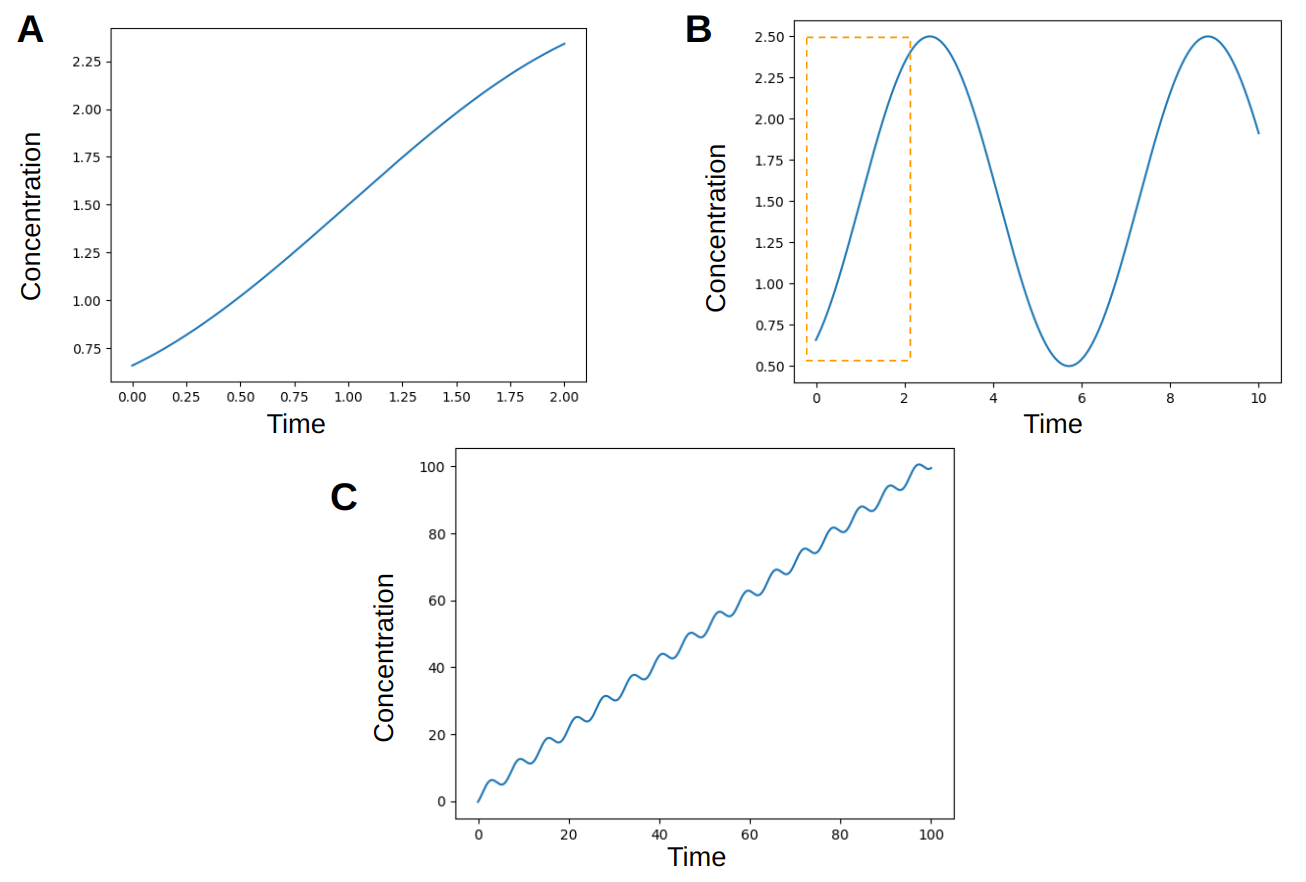
\includegraphics[width=15cm]{images/infinity.png}
    \captionof{table}{Challenges in testing for concentrations that approach infinity with time series data. (A) Appears to approach infinity, but is in fact an oscillator, as depicted in (B). The orange box shows the time period plotted in (A). (C) A species may decrease in concentration at some points, but still approach infinite concentration.}
    \label{fig:infinity}
\end{center}


\section{Specific Changes in Model Variables}
Due to range variety of systems biology models, some credibility tests may be specific to the model in question. These tests would be customized by the model developer and would relate to the behavior expected in the model of interest. One such test might verify that key species in the model behave as expected when other model variables are changed. For example, if the concentration of ATP were to increase, the concentration of ADP might be expected to decrease. If such a decrease were not present after an increase in ATP, it might indicate an error in the model or a peculiarity in the model's function, either of which would imply that the model is less credible. 

These tests are not limited to species concentrations. Changes in enzyme concentration or substrate might be expected to increase reaction rates or flux. For example, and increase in enzyme concentration should produce an increase in the associated reaction's rate. Increasing glucose concentration should increase glycolytic rates.

These tests would be defined by the user, but the proposed software would automatically create these tests upon definition of the parameters in question and the expected result. The result of these customized tests and the tests themselves would be recorded in a credibility report file and a test file respectively to be included with the model upon dissemination.

Although these test have yet to be developed, some testing techniques are already under consideration. In the case of expected concentration changes with respect to another variable (e.g. increases in ATP resulting in decreases of ADP), it may be useful to compute the derivatives of existing time series data. The user could specify the species in question (e.g. ATP and ADP) and indicate their expected correlation (negative in this case). The test software would then numerically compute the derivatives across the time series data and report the percent of data that demonstrated the expected correlation.

These tests may also make use of the ``events" feature in the antimony model description language~\cite{Smith2009}. An instantaneous change in species concentration or rate can be programmed into the model to take place at a specific time in the simulation. For example, an event could be added that would cause glucose to instantaneously double in value. The test could check if the rate of conversion from glucose to glucose 6-phosphate increases as well as other downstream reactions at that moment. 


\section{Bounds Checking}
Checking that certain species concentrations stay within a specified bounds could also be a model specific credibility test. The user would input an upper and lower bounds for a specific species concentration. The simulation would  be run and the time series data examined to ensure that the species concentration did not deviate from the specified range. 

These tests would likely be based on known biological properties. For example, normal blood glucose concentrations typically fall between 3.5 and 5.5 mM~\cite{Guemes569}. ``Normal" blood glucose concentrations vary among individuals as well as the labs measuring these concentrations. To be generous, a user might specify that the glucose concentration in a model of blood glucose dynamics be no less than 2 mM and no greater than 8 mM. A model producing a glucose concentration beyond this range might have an error in structure or parameter value that renders it less  credible. This is of course a very simple example and one might expect a modeler building a blood glucose model would surely examine the output of the primary species of interest, but even in this simple case, such a test could serve as a tool to ensure that the model was disseminated without error or that the numerical algorithms are functioning as they should. An addition parameter sensitivity test (described in chapter 7), might point a user to the parameters that may be responsible for any errors in concentration bounds.





\section{Infrastructure}
Implementing these test will require some additional standardization in file structure. As discussed in chapter 3, COMBINE archives are standardized sip files that contain all necessary files and data required to completely reproduce a systems biology model~\cite{schreiber_specifications_2020}. A credibility testing software could make use of these standardized formats to access models and any associated files. The test system could output a credibility report to be stored in the COMBINE archives for ease of access upon dissemination.

The proposed credibility test suite could also make use of SED-ML (Simulation Experiment Description Markup Language)~\cite{bergmann_simulation_2018,Smith2021simulation, bergmann_combine_2014}, a language developed to describe model simulations. Model developers may already have already created some tests for their models, which could be included in the COMBINE archive as SED-ML files. These tests could  be incorporated into the proposed test suite as an additional measure of credibility. A model that can not pass customized tests that were used in development could be considered less credible.

The test suite could also produce a SED-ML file of the simulations performed to test the model. This would provide transparency as to how tests were performed for that specific model and enable a user to independently reproduce the tests or modify them for their own purposes.


\chapter{Verification and Validation}
\section{Validation}
In the context of computational modeling, validation is defined as ``the process of determining the degree to which a simulation model and its associated data are an accurate representation of the real world from the perspective of the intended uses of the model"~\cite{Thacker2004}. Validation is a component of all existing credibility guidelines reviewed in chapter 3 and can be considered a principal component of any credibility testing suite. Unfortunately validation data or evidence is often omitted from published models, including those curated in databases. In cases where validation was performed, it is often only mentioned in passing in the model's associated research article.  Given its importance model credibility, validation data and evidence should be readily available to third parties in a format that easily allows for confirmation and reproduction. Examining and potentially reproducing model validation may be of interest to users, reviewers, and publishers alike. 

The proposed credibility test suite could support validation testing by allowing users to include validation data sets in the COMBINE Archive. In the shot term, The format of this data might be standardized to allow the test suite to simulate the model and assess the extent to which the model conforms to the validation set. The user could potentially customize an acceptable level of``non-conformity" or the software could simply report a metric describing the the model's ability to match the validation data. The user could optionally include any additional validation tests they performed to be factored into the credibility assessment. Validation tests might be included as python scripts and expected results, python unit tests, or SED-ML files with expected outputs.  The results of these validation tests would be factored in to a credibility score or assessment and included in a credibility report. 

However, it is often the case that systems biology modelers do not wish to write validation tests. The longer term vision for this feature would be a software system with a user friendly interface that would allow modelers to decide how a given model is validated and automatically produce tests to validate the model as specified. Options might include what variable are validated, at what values, and with what data. Validation data might come in the form of time course data, steady-state data, or perturbation data. In addition to validation results, the custom validation tests would be outputted as SED-ML files and python scripts so that users and third parties could easily see exactly what validation tests were performed and reproduce them if desired. For model developers, these test may guide their development process or serve as templates for additional customized validation tests. 




\section{Verification}

Model verification is also a recurring theme in model credibility across disciplines. Verification is defined as ``the process of determining that a model implementation and its associated data accurately represent the developer's conceptual description and specifications" ~\cite{Thacker2004}. In the context of computational modeling, a significant portion of verification consists of static tests, such as checking for typos in rate laws and species name, syntax errors in code, that all parameters are initialized. As static tests are beyond the scope of this proposal, the credibility test suite will perform dynamic verification tests. In the future the proposed dynamic verification tests may be combined with static verification tests in a single model testing software package.

In practice, dynamic verification tests entail testing if the underlying numerical algorithms have been implemented correctly. One way to test this is to check if the model produces the same results when identical simulations are run on different platforms (such as Tellurium~\cite{Choi2018} and COPASI~\cite{Hoops2006}) and operating systems (such as MacOS, Windows, and various Linux distributions). The proposed verification tests will make use of BioSimulations, a user-friendly web applications provides access to a number of different simulation tools and containerized interfaces to each version of each tool~\cite{Shaikh2022}. The credibility assessment software will automatically link to the BioSimulations wed page to simulate the model using several different tools and operating systems. A later iteration of this project could allow users to customize which versions, tools, operating systems, they wish to use for verification. The model would be considered more credible if its outputs are consistent across a variety of platforms.  BioSimulations can also automatically generate reports which could be directly included in the proposed software's credibility assessment report or simplified for brevity. 



\chapter{Sensitivity and Uncertainty Analysis}

\section{Introduction}
A major aspect in model credibility is uncertainty, which appears in many of the credibility guidelines described in chapter 3. The more uncertain a result is, the less credible it is. Uncertainty analysis is performed to investigate the uncertainty in a model's output resulting from uncertainty in parameter inputs~\cite{Marino2008}. Model outputs that depend strongly on parameters with high uncertainty yield less credible predictions. Sensitivity analysis assesses how variations in a model's outputs can be apportioned to different input sources~\cite{Saltelli}. This is illustrated in figure \ref{fig:sensitivity}. Input uncertainty (in this case parameter uncertainty) lies on the X-axis as an inverted probably distribution function. The Y-axis depicts model output as a probability distribution functions. The less uncertain model (blue) has a lower standard deviation compared to the more uncertain result in green. The green line illustrates the relationship between an input parameter with high sensitivity, where a scan across the parameters probability distribution function yields a wider range of model outputs compared to a scan across a less sensitive parameter.  



\begin{figure}
    \centering
    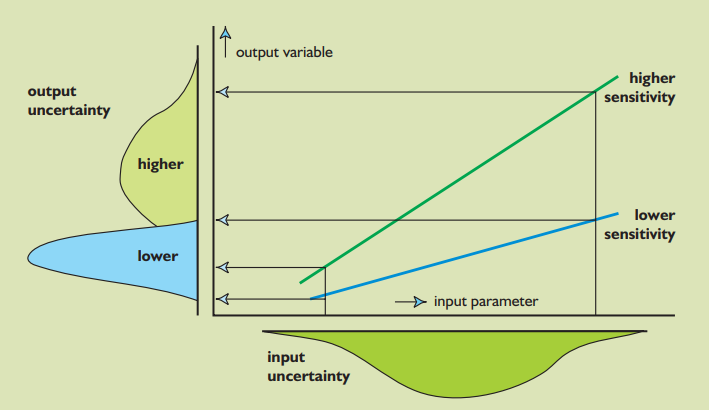
\includegraphics[width=13cm]{images/sensitivity_uncertainty.png}
    \captionof{figure}{The relationship between parameter sensitivity and output uncertainty. In highly sensitive parameters, parameter uncertainty leads to larger output uncertainty and reduced credibility. (Image from Loucks \textit{et al.}~\cite{Loucks2005}, originally published by W. Lal, 1995~\cite{Lal1995}. }
    \label{fig:sensitivity}
\end{figure}

Clearly, highly sensitive parameters that are not known with certainty (as is usually the case) lead to more uncertainty in model results and therefore reduced credibility. There are two reasons that parameter sensitivity should be considered from a credibility perspective. First, in nature, it is unlikely that there is a single ``true" value of a parameter. It is more likely that parameters vary over ranges in different cell types, cellular environments, and genetic variants~\cite{Zi2008}. Second, many biological model display ``sloppy" sensitivity spectra, meaning that most parameters can be varied with minimal effect on the result. In other words, a model output can be predictive and relatively certain despite high uncertainty in parameters~\cite{Gutenkunst2007}.

Although model output uncertainty is more directly indicative of credibility compared to parameter sensitivity, uncertainty analysis is significantly more complicated in terms of implementation, variety of techniques, and computational expense. So while high parameter sensitivity does not necessarily indicate low credibility, it may be useful to highlight highly sensitive parameters so that (1) they can be corrected in the case of a simple mistakes, (2) further and clarified explored experimentally, and (3) model output uncertainty can be apportioned to specific parameters. The third aim of this proposal is to build software to automate simple parameter sensitivity analyses in order to highlight highly sensitive parameters that most contribute to output uncertainty. 



\section{Sources of Parameter Uncertainty}
Computational  modeling has proved useful across a variety of scientific and engineering fields, but modeling applications in biology face unique challenges with parameterization. For example, when modeling systems in classical physics, parameters are often based on physical laws with well established physical constraints. Similarly, in engineering, individual model components are typically well characterized and their interactions known. Computational systems biology faces additional challenges in parameterization due to the reliance on \textit{in vitro} measurements. These measurements can vary due to differences in the biochemical environment and regulatory mechanisms that were not accounted for~\cite{Vanlier2013}. Additionally, these measurements can be expensive and time consuming, resulting in a paucity of data. Combined with the complexity of biological models, this lack of data leads to high uncertainty in inferred parameter values and consequently, poorly constrained and uncertain model predictions.
Although many techniques exist for analyzing parameter sensitivity~\cite{Vanlier2013, Zi2011, vanMourik2014, Volodina2021}, the proposed research will initially explore relatively simple and computationally inexpensive techniques in an effort to make a broadly applicable and user-friendly tool to identify potentially problematic parameter sensitivities.

\section{One-at-a-Time (OAT) Sensitivity Analysis}

There are many techniques to assess the sensitivity of parameters in computational models. A complete exposition of sensitivity analysis and techniques is beyond the scope of this proposal, so discussion will be limited to the relatively simple one-factor-at-a-time analysis. Changing one-factor-at-a-time (OAT) to see how it affects the output is one of the simplest and most common approaches to sensitivity analysis. OAT involves changing an input variable slightly while keeping all others unchanged, measuring the model's output, returning the variable to its baseline value and then repeating for all other input variables. Sensitivty can then be measured by examining changes in the output, usually by partial derivatives, $\partial Y_j/ \partial X_i$, where the change in output $Y_i$ is compared to a change of input $X_i$. This is referred to the sensitivity of $Y_j$ versus $X_i$~\cite{Saltelli}. 

This is the technique that the simulation software RoadRunner uses to quickly asses sensitivity in systems biology models~\cite{Somogyi2015}. RoadRunner defines two types of sensitivity, systems and global, based on metabolic control analysis (MCA)~\cite{RoadRunnerdocs}. Although MCA was originally developed to study metabolic networks, it can also be applied to other biological networks such as cell signaling, genetic networks, and others~\cite{Zi2011}.  Local sensitivity is defined as $\frac{\partial v}{\partial S}\frac{S}{v}$ where $v$ is a reaction rate and $S$ is an effector of the reaction (typically a species that influences the reaction as a substrate, inhibitor, catalyst etc). This metric describes how a change in a reaction's effector species concentration effects the reaction's rate. This metric is scaled, representing approximately $\frac{\%S}{\%v}$

System sensitivities are described by control coefficients, each of which has two forms, flux and concentration~\cite{RoadRunnerdocs}. The flux control coefficient measures how sensitive a reaction's flux is to changes in the reaction rate, usually performed by changing and enzyme concentration. This is defined as   where $E$ is an enzyme concentration and $J$ is a reaction's flux. Similarly, the concentration control coefficient measures how a change in reaction rate (i.e. enzyme concentration) effects a given species concentration, $\frac{\partial S}{\partial E}\frac{E}{S} \approx \frac{\%S}{\%E}$.

As a simple preliminary step, the proposed software will make use of these built in functions to measure local and systems sensitivity, where appropriate. Due to the variety of models, it is likely that not all high sensitivities indicate decreased credibility. For example, a signaling cascade might be particularly sensitive to a species concentration.  Similarly, the amount of ``acceptable" sensitivity may vary from model to model. For these reasons, the preliminary sensitivity assessment will likely be excluded from any quantitative credibility scoring system, but will be included in a credibility report to alert the user to particularly high sensitivities so they can be verified, corrected, or further assessed.

\section{Weaknesses of OAT Sensitivity Analysis}

A possible weakness of this approach, as the name implies, is that sensitivity is measured by perturbing a single variable. It is possible that the combination of two or more parameters perturbed slightly at the same time would dramatically affect the model's output, however testing these combinations is not feasible for the software proposed here, designed to do a coarse grain assessment of a model's general credibility. If this avenue were to be pursued in more detail, it may be possible to implement these features or create a separate software package designed for sensitivity testing. If this were the case, the user might choose the experimental design and ranges over which parameters are tested. 

Additionally, the utility of sensitivity analyses may depend on the identifiability of model parameters. If models are calibrated and well-constrained with large experimental data sets, sensitivity analysis can be highly useful in pinpointing the most influential parameters which should be investigated further. If models are ``sloppy," as is often the case, it is difficult to determine the parameters by fitting to experimental data. In these cases, sensitivity analysis may be a useful tool to gauge model output uncertainty, but the information may not be sufficient to identify parameters that should be studied further~\cite{Zi2011}. In any case, the purpose of including sensitivity analysis in this tool is to serve as a preliminary assessment of result uncertainty. Extensive sensitivity testing and result uncertainty quantification is beyond the scope of this research, although a python package implementing more complex sensitivity and uncertainty analyses for systems biology models may prove useful to the modeling community.


\chapter{Summary}

As computational models become increasingly important in decision-making, so too does model credibility. Although many efforts have been made in systems biology to create standards that ensure model reproducibility, to date, no standards exist to promote credibility. In other industries, such as aerospace, medical devices, and pharmaceuticals, preliminary credibility guidelines have been developed to steer model creators towards making credible models. Owing to the range of applications and models in these fields, these credibility guidelines are largely qualitative and highly subjective. Fortunately, computational systems biology models are of relatively small scope and already rely on several standards describing model description, annotation, simulation, and dissemination. The purpose of the proposed research is to standardize systems  biology model credibility with a software tool that automatically assess and scores the credibility of models. 

This research is broken down into three aims: (1) to create dynamic tests to assess systems biology model credibility, (2) to create tools to verify and validate models, and (3) to automate simple parameter sensitivity tests as a proxy for result uncertainty. The proposed tests and possible implementations are summarized in table \ref{table:sensitivity}. It is likely that as the research progresses, more tests and implementations will be added to this list. 

The proposed research is expected to result in two first author publications, to be submitted by June 2024. The first will highlight the need and uses of the software, introduce the tests to be performed, and provide a simple demonstration of an early implementation of the software on simple models. The second publication will introduce the fully developed software and demonstrate its functionality with several published models.

\begin{figure}
    \centering
    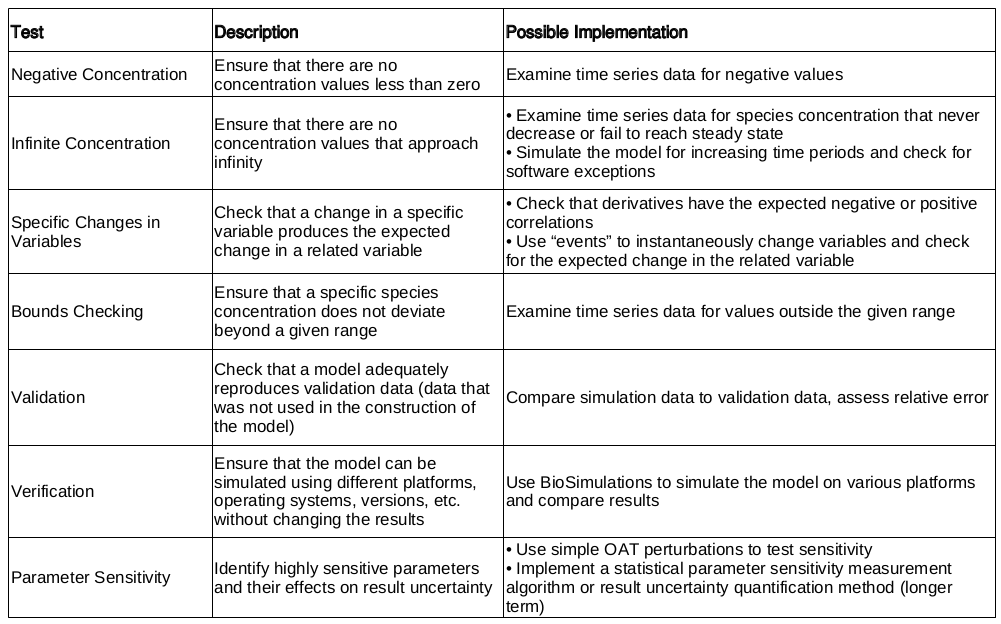
\includegraphics[width=19cm]{images/testSummary.png}
    \captionof{table}{Summary of proposed tests and possible implementations.}
    \label{table:sensitivity}
\end{figure}



% Bibliography
\bibliographystyle{unsrt}
\bibliography{researchbib}
\end{document}


